\chapter{Segmentación con redes neuronales}
\label{chap:Segmentacion con redes neuronales}
\Abstract{En este capítulo se van a desarrollar tres técnicas diferentes para la detección de piezas LEGO. Las técnicas desarrollados son R-CNN, Faster R-CNN y YOLO. A su vez, para cada una de estas se desarrollaran dos redes basadas en LEGONet y LEGO16.}

El objetivo final de este proyecto es la implantación de un sistema de detección de piezas de LEGO de forma que un brazo robótico pueda identificar y recoger dichas piezas. En el \autoref{chap:Segmentacion con mascaras de color} ya se ha desarrollado un método capaz de realizar dicha tarea pero debido a la tecnología empleada, el sistema presenta demasiados falsos positivos y solo es capaz de trabajar bajo condiciones ideales. Por ello se ha decidido emplear las últimas tecnologías para la detección de objetos en imágenes. Y en la actualidad los detectores de objetos más modernos se basan en redes neuronales convolucionales. Para su desarrollo es común y recomendado partir de un clasificador ya entrenado y reusarlo con el propósito de convertirlo en un detector de objetos.

En el \autoref{chap:Clasificacion con redes neuronales} se ha desarrollado dos clasificadores diferentes con el fin de ser usados para el desarrollo de múltiples detectores de imágenes. Se van a desarrollar un total de seis detectores de objetos empleando diferentes tecnologías y se compararan entre sí. Para facilitar el desarrollo del proyecto, las redes neuronales se han desarrollado de forma escalonada en función de su nivel de complejidad. Empezando por la red más simple y terminando por la red más compleja. Por nivel de complejidad nos referimos a la complejidad de las tecnologías empleadas y a su dificultad de compresión y no al número de capas que constituyen la red neuronal. Pero antes de desarrollar estas redes, es necesario contextualizar el proyecto. A continuación, se va a mostrar de que datos se parte y como se van a entrenar dichas redes neuronales.

\section{Preparativos para el entrenamiento y evaluación}
\label{sec:Preparativos para el de entrenamiento detectores}
Para poder entrenar detectores de objetos basado en clasificadores es necesario disponer de una buena base de datos de la que puedan aprender y ser evaluados. En esta sección se van a desarrollar ambas bases de datos.

\subsection{Entrenamiento}
\label{subsec:entrenamiento}
Para el desarrollo de este proyecto se va a emplear aprendizaje supervisado lo cual implica que toda la información debe haber sido preparada, etiquetada y analizada para que la red pueda aprender de esta. En el caso de los detectores de objetos esta información consta de dos objetos. En primer lugar, la imagen de la que se desea aprender y en segundo lugar, las posiciones de los objetos que debe de detectar y el tipo de objeto que es. Esta posición se indica en forma de \textit{bounding box}, es decir, se dan la posición y dimensión de un rectángulo que contiene dicho objeto. Los \textit{bounding boxes} se dan en píxeles con forma de un vector de dimensión cuatro. Se da la posición en ejes x e y de la esquina superior izquierda y el alto y ancho del rectángulo.

Con la ayuda de MATLAB e \textit{imageLabeler} se ha preparado un conjunto de imágenes clasificadas y etiquetadas para llevar acabo el entrenamiento de las redes neuronales. En total se han preparado y etiquetado un total de 346 imágenes con un total de 981 piezas de LEGO. A continuación, se muestra en la \autoref{fig:entrenamiento mosaico} algunas de las imágenes empleadas para el entrenamiento.

\begin{figure}[ht]  %Imágenes para el entrenamiento
  \subfloat{
	\begin{minipage}[c][1\width]{0.3\textwidth}
	   \centering
	   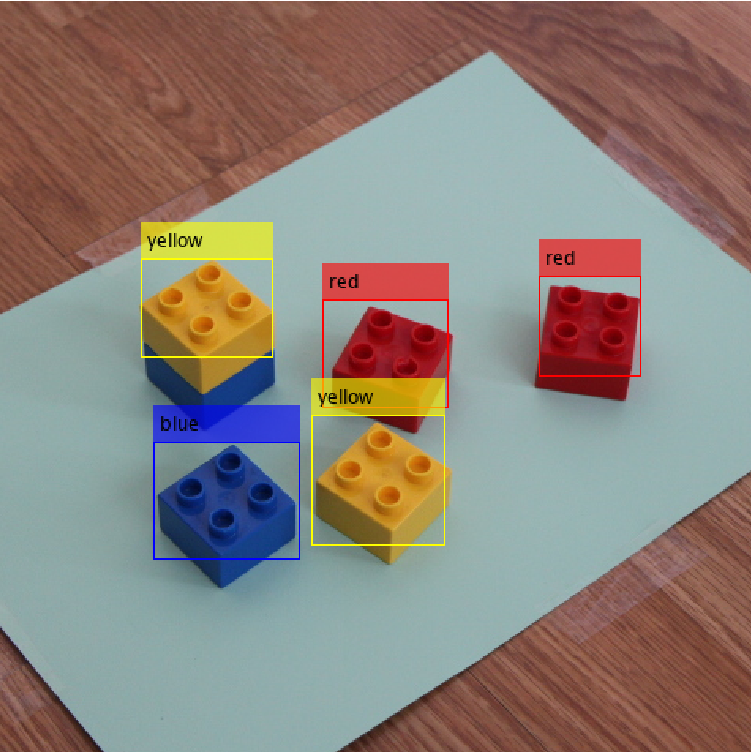
\includegraphics[width=1\textwidth]{Segmentacion con redes neuronales/Entrenamiento/entrenamiento1.png}
	\end{minipage}}
  \hfill	
  \subfloat{
	\begin{minipage}[c][1\width]{0.3\textwidth}
	   \centering
	   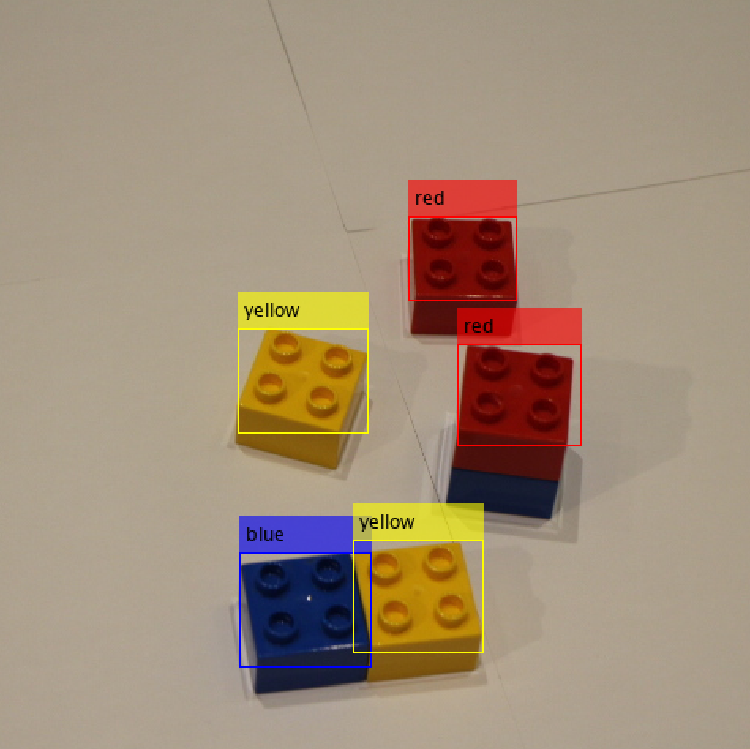
\includegraphics[width=1\textwidth]{Segmentacion con redes neuronales/Entrenamiento/entrenamiento2.png}
	\end{minipage}}
  \hfill	
  \subfloat{
	\begin{minipage}[c][1\width]{0.3\textwidth}
	   \centering
	   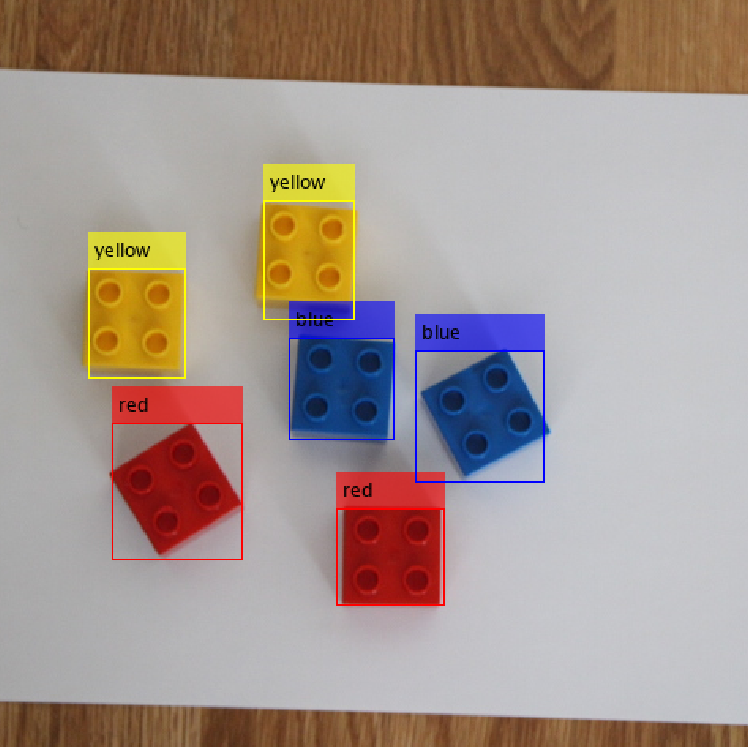
\includegraphics[width=1\textwidth]{Segmentacion con redes neuronales/Entrenamiento/entrenamiento3.png}
	\end{minipage}}
\caption{Imágenes empleadas para el entrenamiento de segmentación con redes neuronales}
\label{fig:entrenamiento mosaico}
\vspace{-5pt}
\end{figure}

Para el entrenamiento de redes neuronales es recomendable tener una buena y amplia base de datos sobre la que la red pueda aprender. Por ello, para aumentar aún más el número de imágenes disponibles, se ha acudido a diversas herramientas.

\begin{itemize}
\item Transformación del color: se ha generado simultáneamente variaciones del contraste, matiz y brillo de forma aleatoria pero dentro de unos límites. Al aplicar estas modificaciones a las imágenes originales se consigue variar notablemente la imagen respecto a la original.
\item Espejo: se han reflejado las imágenes de tres formas posibles. Se han reflejado en el eje x, el eje y y respecto a ambos ejes a la vez.
\item Recortes: se han realizado de forma aleatorio, pero dentro de unos límites, recortes de las imágenes originales para crear nuevas.
\item Deformaciones: se han generado pequeñas deformaciones de forma de las imágenes originales para crear nuevas. Las deformaciones se encuentran dentro de unos límites.
\end{itemize}

Aplicando estas técnicas, se ha conseguido aumentar notablemente en el número de imágenes pasando de 346 a 2.076 y de 981 piezas de LEGO a 5.886. Es decir, se ha conseguido incrementar seis veces el número de imágenes y de piezas.

\begin{figure}[ht]  %Aumento de imágenes
  \subfloat{
	\begin{minipage}[c][1\width]{0.3\textwidth}
	   \centering
	   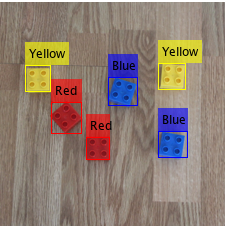
\includegraphics[width=1\textwidth]{Segmentacion con redes neuronales/Entrenamiento/augmented1.png}
	\end{minipage}}
  \hfill	
  \subfloat{
	\begin{minipage}[c][1\width]{0.3\textwidth}
	   \centering
	   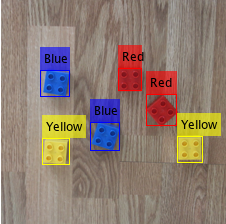
\includegraphics[width=1\textwidth]{Segmentacion con redes neuronales/Entrenamiento/augmented2.png}
	\end{minipage}}
  \hfill	
  \subfloat{
	\begin{minipage}[c][1\width]{0.3\textwidth}
	   \centering
	   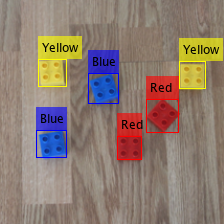
\includegraphics[width=1\textwidth]{Segmentacion con redes neuronales/Entrenamiento/augmented3.png}
	\end{minipage}}
\caption{Aumento del número de imágenes para el entrenamiento}
\label{fig:RCNN augmentation}
\vspace{-5pt}
\end{figure}

\begin{table}[ht]
  \centering
    \begin{tabular}{|l|r|}
    \hline
    \multicolumn{2}{|c|}{Total de piezas}\\
    \hline
    Rojo & 2106 \\
    \hline
    Azul & 1818 \\
    \hline
    Amarillo & 1962 \\
    \hline
    \end{tabular}%
    \caption{Base de datos para el entrenamiento de detectores de objetos}
  \label{tab:RCNN imagenes}%
\end{table}%

Todo el entrenamiento se ha llevado a cabo en un ordenador personal equipado con un i7 4790K, 16GB de memoria RAM y una tarjeta gráfica Nvidia Geforce GTX970 con 4GB de VRAM. Teniendo en cuenta las limitaciones por \textit{hardware} y tiempo, se han realizado múltiples entrenamientos con diferentes opciones de entrenamiento para obtener los mejores resultados con cada red.

\subsection{Evaluación}
\label{subsec:evaluacion}
Para comprobar la eficacia de las redes creadas, se ha desarrollado un \textit{script} con la ayuda de MATLAB para determinar su capacidad de para identificar piezas y la precisión con las que la detecta. En este \textit{script} se han analizado 74 imágenes con más de 380 piezas de LEGO. Y con el fin de obtener un análisis riguroso y que refleje la capacidad de este método ante diversas condiciones, se han seleccionado fotos con múltiples ángulos y escenas. A continuación, se muestra algunas de las imágenes usadas para la evaluación:

\begin{figure}[ht]  %evaluación redes
	\centering
	\includegraphics[width=0.8\textwidth]{Segmentacion con redes neuronales/Entrenamiento/evaluacion.png}
	\caption{Muestra de imágenes para la evaluación de redes neuronales}
	\label{fig:evaluacion redes}
\end{figure}

Con la ayuda del \textit{script} se han podido obtener cuatro parámetros que permiten evaluar los resultados. En primer lugar, se ha obtenido la tasa de fallos y el número de falsos positivos por imagen para cada una de las clases. Y a continuación se ha evaluado la precisión de las piezas encontradas y la exhaustividad, que es la relación entre verdaderos positivos y la suma de verdaderos positivos y falsos negativos.

%%%%%%%%%%%%%%%%%%%%%%%%%%%%%%%%%%%%%%%%%%%%%%%%%%%%%%%%%%%%%%%%%%%%%%%%%%%%%%%%%%%%%%%%%%%%%%%%%%%%%%%%%%%%%
%%%%%%%%%%%%%%%%%%%%%%%%%%%%%%%%%%%%%%%%%%%%%%%%%%%%%%%%%%%%%%%%%%%%%%%%%%%%%%%%%%%%%%%%%%%%%%%%%%%%%%%%%%%%%
\newpage
\section{R-CNN}
Tal y como se ha explicado en la \autoref{subsec:RedesNeuronalesConvolucionales}, R-CNN (\textit{Region-proposal Convolutional Neuronal Network}) es un sistema basado en un clasificador y el sistema de propuesta de regiones. La idea surgió porque previamente a este sistema, la solución para poder detectar objetos consistía en correr un clasificador por toda la imagen variando el tamaño del clasificador. Este método se conoce como ventana flotante y suponía una gran carga computacional ya que se tenía que correr el clasificador numerosas veces para analizar una sola imagen. Pero en  surgió el método R-CNN \cite{RCNN}, este consiste en la propuesta de 2000 zonas con posibilidades de contener un objeto. De esta forma se limitaba el número de regiones mejorando así el rendimiento.

	\begin{figure}[ht]
		\centering
		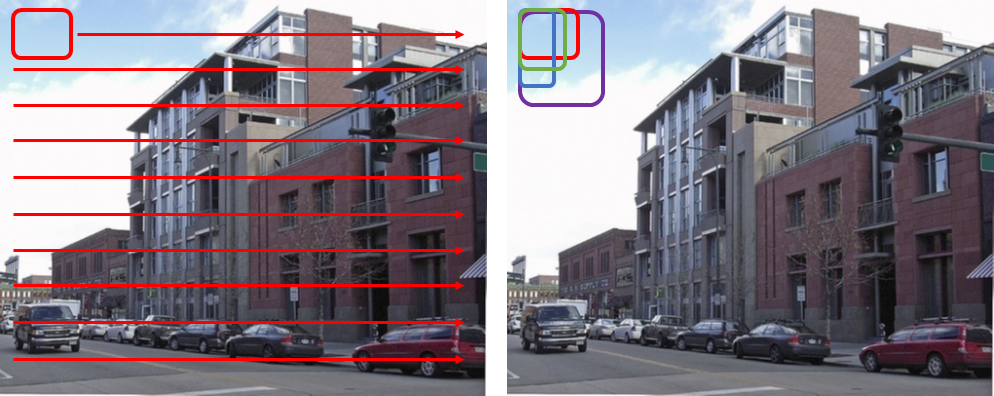
\includegraphics[width=0.7\textwidth]{Segmentacion con redes neuronales/R-CNN/sliding windows.png}
		\caption{Demostración del concepto de ventana flotante (Fuente: \citep{Review_RCNN})}
		\label{fig:R-CNN sliding window}
		\vspace{-5pt}
	\end{figure}
	
	\begin{figure}[ht]
	\centering
	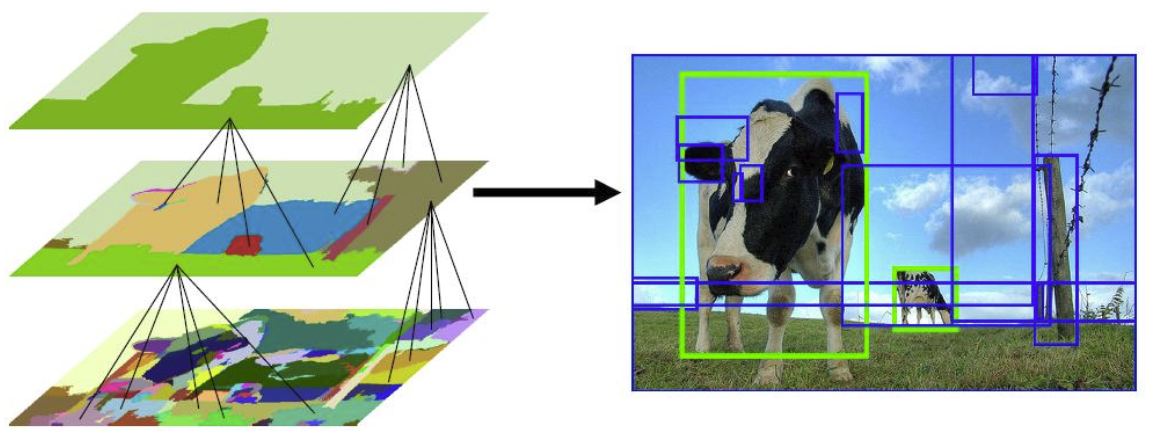
\includegraphics[width=0.7\textwidth]{Segmentacion con redes neuronales/R-CNN/region proposal.png}
	\caption[Estimación de las regiones de interés con R-CNN]{Estimación de las regiones de interés con R-CNN (Fuente: \citep{Review_RCNN})}
	\label{fig:R-CNN region proposal}
	\vspace{-5pt}
	\end{figure}

El proceso de propuesta de regiones se basa en diferentes características de la imagen. Se intenta buscar similitudes de color, texturas, tamaños.... Una vez analizada toda la imagen y obtenidas todas las posibles regiones, estas se analizan y se intenta unir las regiones pequeñas y próximas de forma que se termine con aproximadamente 2000 regiones a analizar.

	\begin{figure}[ht]
	\centering
	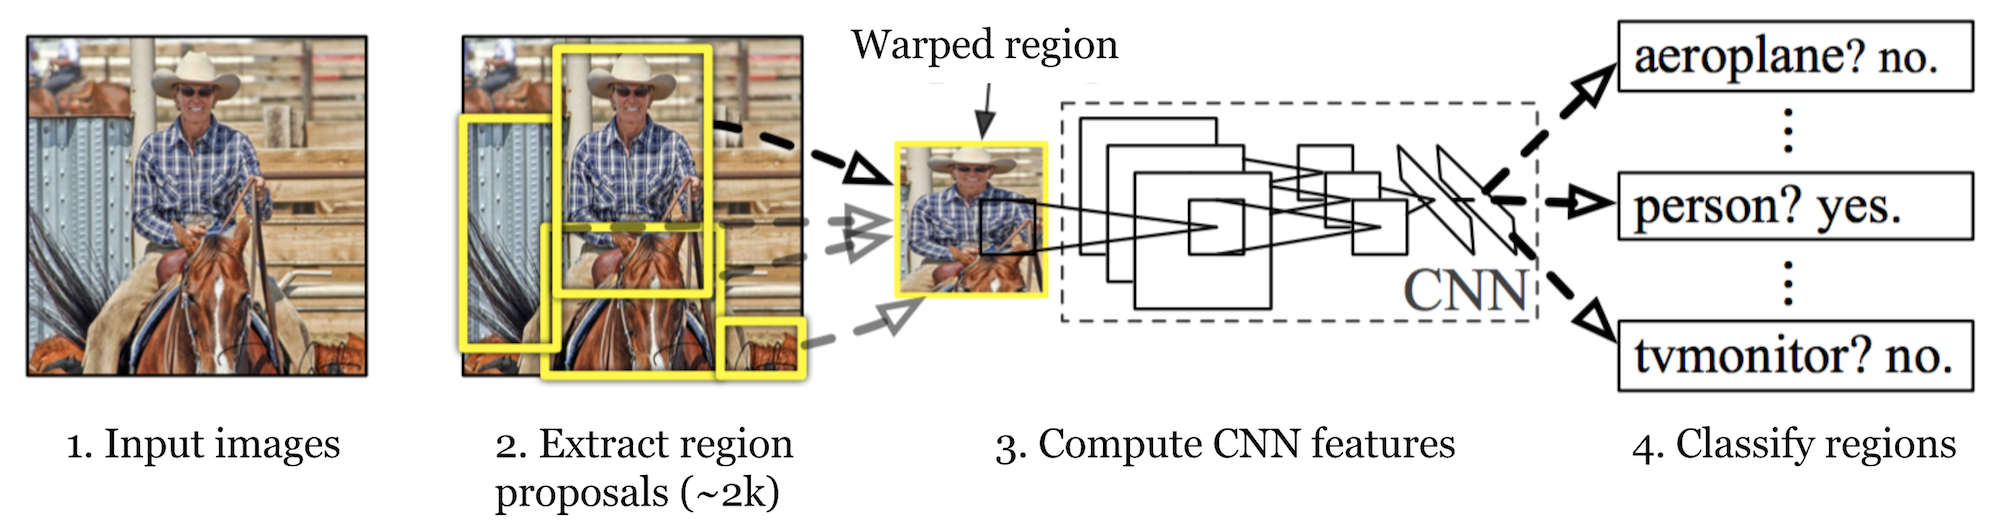
\includegraphics[width=0.7\textwidth]{Segmentacion con redes neuronales/R-CNN/RCNN.png}
	\caption[Representación del funcionamiento de R-CNN]{Representación del funcionamiento de R-CNN (Fuente: \citep{RCNN})}
	\label{fig:R-CNN esquema}
	\vspace{-5pt}
	\end{figure}

Con el objetivo de poder comparar diversas redes neuronales y su evolución en el paso del tiempo, se han desarrollado dos redes tipo R-CNN basadas en dos clasificadores diferentes. Se han usado los clasificadores creados en el \autoref{chap:Clasificacion con redes neuronales} que a su vez están basados en AlexNet y VGG-16.

\subsection{R-CNN basado en LEGONet}
Partiendo del clasificador LEGONet y con la ayuda de MATLAB y una base de datos de imágenes de LEGOS, se ha creado y entrenado un detector de objetos tipo R-CNN.

\subsubsection*{Estructura}
LEGONet esta formada por un total de 25 capas, 60 millones de parámetros y 650.000 neuronas. De las 25 capas, 5 son capas convoluciones, 2 son capas completamente conectadas y entre medias se encuentran capas del tipo \textit{ReLu}, \textit{Batch normalization}, \textit{Max pooling} y \textit{Dropouts}. Para poder ser reutilizado y empleado como detector de objetos, es necesario modificar la estructura y el funcionamiento de la red neuronal.

Como se puede ver en la \autoref{fig:R-CNN esquema}, R-CNN es un proceso definido por dos etapas, la primera etapa es la propuesta de regiones y la segunda es el análisis de dichas regiones con el clasificador. Esto implica que a LEGONet se le va a tener que incluir el proceso de propuesta de regiones y de nuevo, se van a tener que modificar las tres últimas capas para reentrenar al clasificador para distinguir las piezas de LEGO.

\begin{itemize}
\item Capa 23: Completamente conectada (1x1x7) $\rightarrow$ (1x1x4)
\item Capa 24: \textit{Softmax} (1x1x1000) $\rightarrow$ (1x1x4)
\item Capa 23: Salida del clasificador
\end{itemize}

La dimensión de estas nuevas capas es cuatro ya que R-CNN necesita también incluir la clase fondo para el caso en que no detecte nada en alguna de las regiones propuestas. Con estos cambios, la nueva estructura se puede ver en la \autoref{fig:R-CNN_LEGONet estructura}

\begin{figure}[ht]  %LEGONet
	\centering
	\includegraphics[width=0.95\textwidth]{Segmentacion con redes neuronales/R-CNN/RCNN_LEGONet.pdf}
	\caption{Estructura de R-CNN basado en LEGONet}
	\label{fig:R-CNN_LEGONet estructura}
\end{figure}


\subsubsection*{Entrenamiento}
\label{subsubsec:Entrenamiento R-CNN_LEGONet}
Para el entrenamiento de esta red se ha usado la base de datos diseñada en la \autoref{sec:Preparativos para el de entrenamiento detectores}. Esta base de datos consta de un total de 2.076 imágenes con un total de 5.886 piezas de LEGO. Se han realizado numerosas pruebas de entrenamiento y se ha descubierto que las mejores opciones de entrenamiento son las mostradas en la \autoref{tab:RCNN options}.

\begin{table}[ht]
  \centering
    \begin{tabular}{|l|c|}
    \hline
    \multicolumn{2}{|c|}{Opciones de entrenamineto} \\
    \hline
    Solver & \multicolumn{1}{l|}{Stochastic Gradient Descent with Momentum (SGDM)} \\
    \hline
    Momentum & 0.9 \\
    \hline
    Initial Learn Rate & 1.00E-04 \\
    \hline
    Learn Rate Schedule & piecewise \\
    \hline
    Learn Rate Drop Factor & 0.5 \\
    \hline
    Learn Rate Drop Period & 35 \\
    \hline
    L2Regularization & 0.004 \\
    \hline
    Max Epochs & 400 \\
    \hline
    Mini Batch Size & 200 \\
    \hline
    Shuffle data & every epoch \\
    \hline
    \end{tabular}%
  \caption{Opciones de entrenamiento de R-CNN basado en LEGONet}
  \label{tab:RCNN options}%
\end{table}%

\subsubsection*{Resultados}
Con la ayuda del \textit{script} definido en la \autoref{subsec:evaluacion}, se han podido obtener cuatro parámetros que permiten evaluar la capacidad de esta red: tasa de fallos, falsos positivos por imagen (FPPI), precisión de los \textit{bounding boxes} y la exhaustividad. Al correr un detector de objetos existen múltiples parámetros a definir por el usuario que marcan el comportamiento de la red. Se ha evaluado la red con todas las posibles combinaciones de parámetros lógicas y se ha determinado el mejor rango de funcionamiento de la red. Estos parámetros son el nivel de superposición de las \textit{bounding boxes} y el límite de incertidumbre aceptable para determinar que lo detectado es un objeto. Al analizar todos los casos lógicos se han obtenido los resultados mostrados en la \autoref{fig:RCNN LEGONet evaluacion}. En el eje x se puede ver los casos que se han analizado. El umbral de confianza se ha variado desde 0.5 hasta 1 en intervalos de 0.05 y para cada caso se ha evaluado modificando el nivel de superposición entre \textit{bounding boxes}. El nivel de superposición se ha variado entre 0 y 0.5 con intervalos de 0.05.

\begin{figure}[ht]  %Evaluación R-CNN basado en LEGONet
	\centering
	\includegraphics[width=1\textwidth]{Segmentacion con redes neuronales/R-CNN/evaluacion.png}
	\caption{Evaluación de R-CNN basado en LEGONet en función de diversos parámetros}
	\label{fig:RCNN LEGONet evaluacion}
\end{figure}

Analizando estos resultados, se ha determinado que un buen punto de compromiso entre precisión, tasa de fallos y falsos positivos se obtiene con un límite de incertidumbre de 0.95 y un factor de superposición de 0.25. En los resultados mostrados a continuación se ha trabajado en este punto de operación. Tras analizar observamos que todas las gráficas siguen las distribuciones esperadas, al aumentar los falsos positivos hay más posibilidades de detectar la pieza y por ello aumenta la precisión. Al reducir los falsos positivos pasa el efecto contrario. Al reducir los falsos positivos hay mayor probabilidad de no detectar la pieza y al aumentarlos, pasa el caso contrario. Analizando cada caso por separado, se ha llegado a las siguientes conclusiones:
\begin{itemize}
\item Amarillo: El error cometido al detectar las piezas tanto en precisión como en fallos y falsos positivos en bastante pequeño. Y si se observan las gráficas se puede deducir que no han sido numerosos los casos en los que no se han detectado correctamente las piezas y por ello tienen una forma tan rectilínea.
\item Rojo: La tasa de fallos es bastante superior respecto al amarillo y la precisión también baja. El número de falsos positivos por imagen también crece bastante. Analizando las imágenes de forma individual se ha observado que esto se debe a que en varias situaciones el sistema detectaba varias veces la misma pieza roja.
\item Azul: El azul es una situación intermedia entre el rojo y el amarillo. Tiene una precisión bastante elevada y una tasa de fallos baja, pero presenta una mayor número de falsos positivos que el amarillo.
\end{itemize}

Al comparar estos resultados con los previamente obtenidos en segmentación con máscaras de color (\autoref{chap:Segmentacion con mascaras de color}) observamos la verdadera capacidad de las redes neuronales y por qué representan el futuro. R-CNN destaca por ser mucho más robusto y constante y con un menor número de falsos positivos. Se puede observar una mejor comparación entre todos los métodos en el \autoref{chap:Resultados}.


\begin{figure}[ht]  %Estudio Amarillo
\vspace{-30pt}
  \subfloat{
	\begin{minipage}[c][1\width]{0.49\textwidth}
	   \centering
	   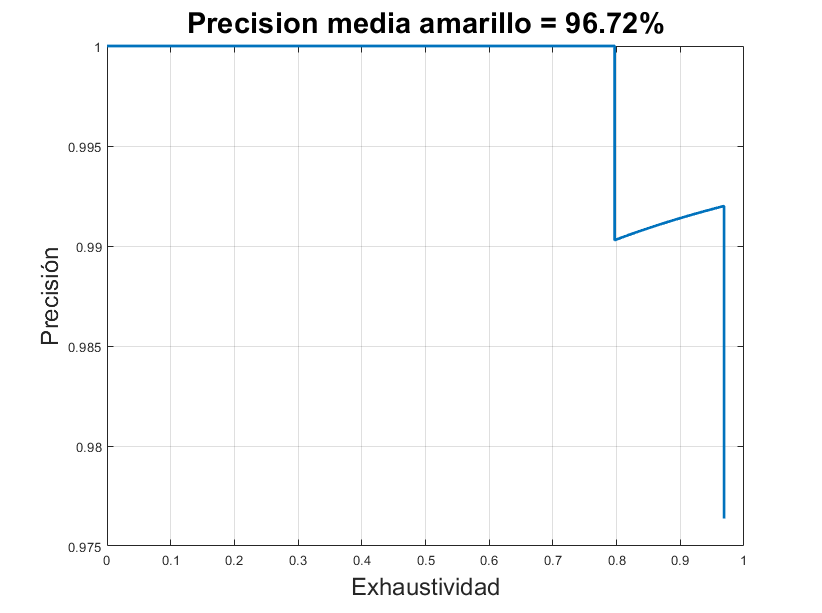
\includegraphics[width=1\textwidth]{Segmentacion con redes neuronales/R-CNN/RCNN precision_yellow.png}
	\end{minipage}}
  \hfill	
  \subfloat{
	\begin{minipage}[c][1\width]{0.49\textwidth}
	   \centering
	   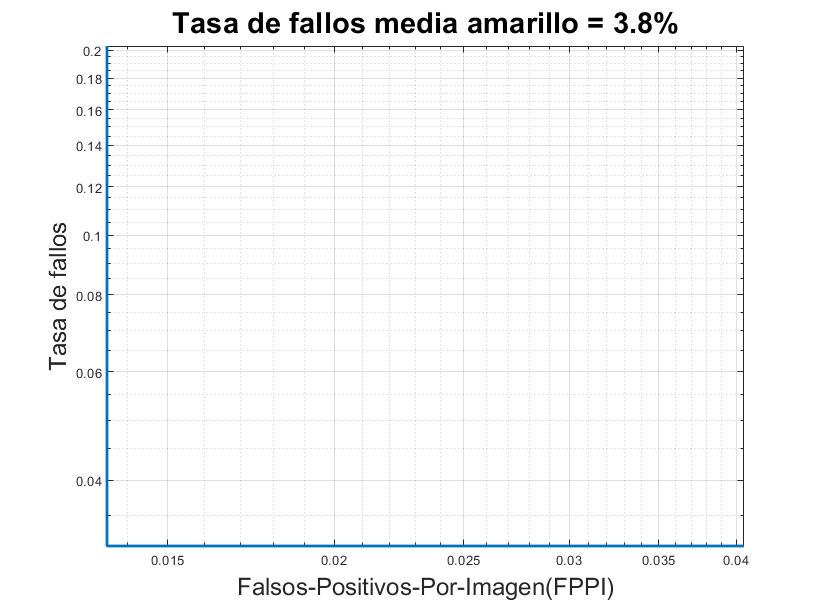
\includegraphics[width=1\textwidth]{Segmentacion con redes neuronales/R-CNN/RCNN miss_yellow.png}
	\end{minipage}}
\vspace{-15pt}
\caption{Estudio de la segmentación por R-CNN al detectar piezas amarillas}
\label{fig:yellow R-CNN}
\end{figure}

\begin{figure}[ht]  %Estudio Rojo
\vspace{-30pt}
  \subfloat{
	\begin{minipage}[c][1\width]{0.49\textwidth}
	   \centering
	   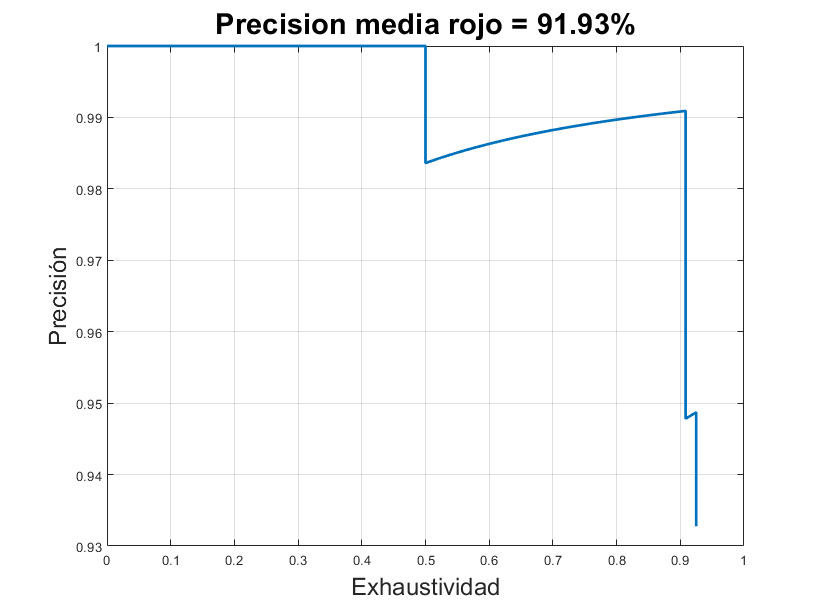
\includegraphics[width=1\textwidth]{Segmentacion con redes neuronales/R-CNN/RCNN precision_red.png}
	\end{minipage}}
  \hfill	
  \subfloat{
	\begin{minipage}[c][1\width]{0.49\textwidth}
	   \centering
	   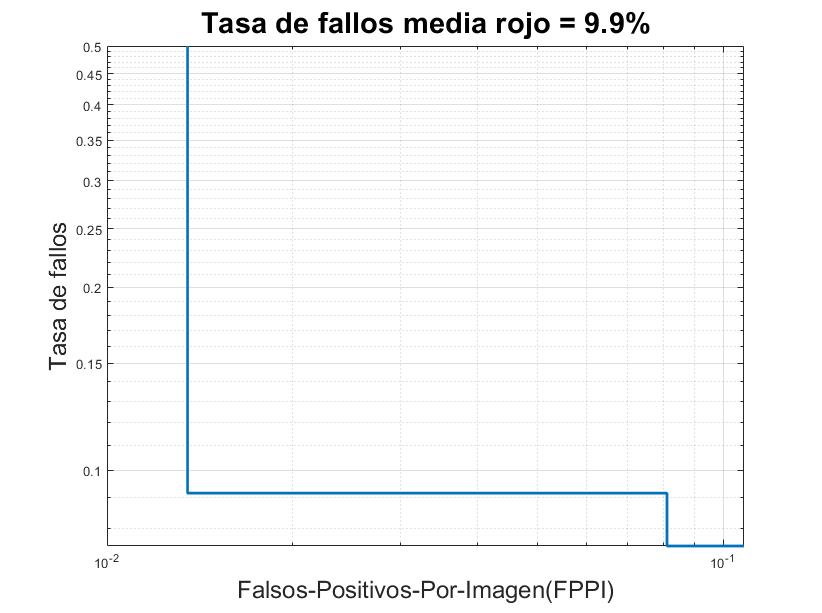
\includegraphics[width=1\textwidth]{Segmentacion con redes neuronales/R-CNN/RCNN miss_red.png}
	\end{minipage}}
\vspace{-15pt}
\caption{Estudio de la segmentación por R-CNN al detectar piezas rojas}
\label{fig:red R-CNN}
\end{figure}

\begin{figure}[H]  %Estudio Azul
\vspace{-30pt}
  \subfloat{
	\begin{minipage}[c][1\width]{0.49\textwidth}
	   \centering
	   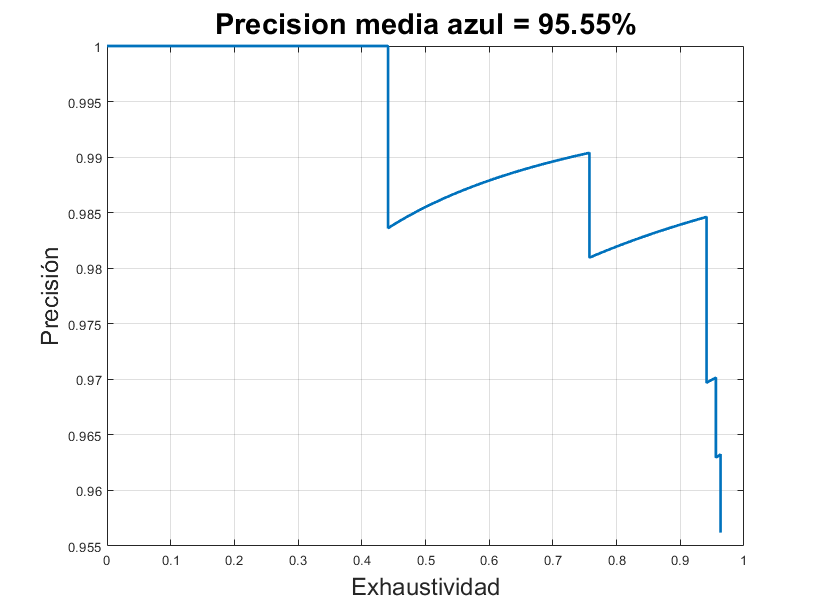
\includegraphics[width=1\textwidth]{Segmentacion con redes neuronales/R-CNN/RCNN precision_blue.png}
	\end{minipage}}
  \hfill	
  \subfloat{
	\begin{minipage}[c][1\width]{0.49\textwidth}
	   \centering
	   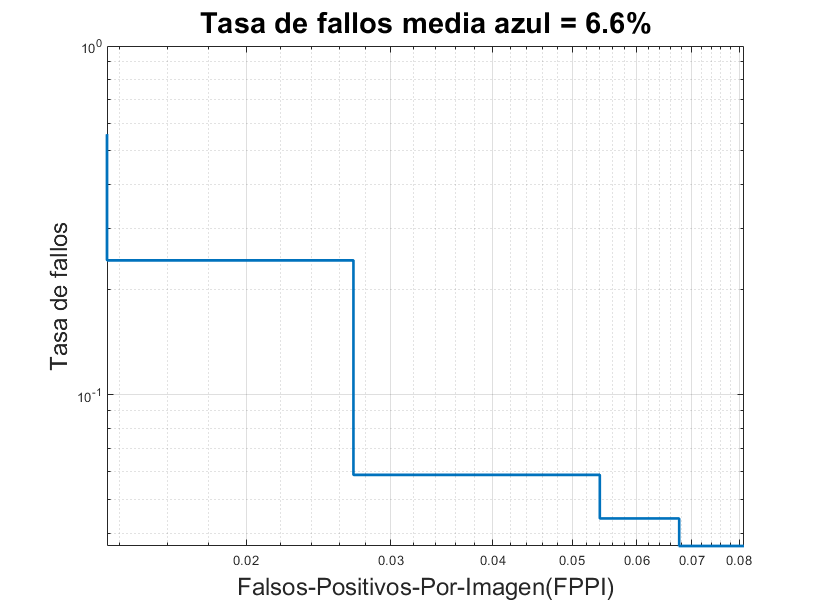
\includegraphics[width=1\textwidth]{Segmentacion con redes neuronales/R-CNN/RCNN miss_blue.png}
	\end{minipage}}
\vspace{-15pt}
\caption{Estudio de la segmentación por R-CNN al detectar piezas azules}
\label{fig:blue R-CNN}
\end{figure}


\subsection{R-CNN basado en LEGO16}
Partiendo del clasificador LEGO16 y con la ayuda de MATLAB y la base de datos de imágenes de LEGOS de la \autoref{subsec:entrenamiento}, se ha creado y entrenado un detector de objetos tipo R-CNN.

\subsubsection*{Estructura}
LEGO16 está formada por un total de 16 capas con pesos y un total de 41 capas, 138 millones de parámetros y 13 millones de neuronas. De las 16 capas, 13 son capas convoluciones, 3 son capas completamente conectadas y entre medias se encuentran capas del tipo \textit{ReLu}, \textit{Max pooling} y \textit{Dropouts}. Para poder ser reutilizado y empleado como detector de objetos, es necesario modificar la estructura y el funcionamiento de la red neuronal.

Como se puede ver en la \autoref{fig:R-CNN esquema}, R-CNN es un proceso definido por dos etapas, la primera etapa es la propuesta de regiones y la segunda es el análisis de dichas regiones con el clasificador. Esto implica que a LEGONet se le va a tener que incluir el proceso de propuesta de regiones y de nuevo, se van a tener que modificar las tres últimas capas para reentrenar al clasificador para distinguir las piezas de LEGO.

\begin{itemize}
\item Capa 39: Completamente conectada (1x1x7) $\rightarrow$ (1x1x4)
\item Capa 40: \textit{Softmax} (1x1x1000) $\rightarrow$ (1x1x4)
\item Capa 41: Salida del clasificador
\end{itemize}

La dimensión de estas nuevas capas es cuatro ya que R-CNN necesita también incluir la clase fondo para el caso en que no detecte nada en alguna de las regiones propuestas. Con estos cambios, la nueva estructura se puede ver en la \autoref{fig:R-CNN_LEGO16 estructura}

\begin{figure}[ht]  %LEGO16
	\centering
	\includegraphics[width=0.95\textwidth]{Segmentacion con redes neuronales/R-CNN/RCNN_LEGO16.pdf}
	\caption{Estructura de R-CNN basado en LEGO16}
	\label{fig:R-CNN_LEGO16 estructura}
\end{figure}

\subsubsection*{Entrenamiento y resultados}
En este proyecto se ha desarrollado la estructura y se han hecho todos los preparativos para el entrenamiento de esta red neuronal, desgraciadamente, debido a limitaciones por \textit{hardware} no se ha podido entrenar y por lo tanto no hay resultados que mostrar. Por suerte, estas limitaciones solo han sucedido en el desarrollo de R-CNN basado en LEGO16 y esto es debido a falta de memoria VRAM.

%%%%%%%%%%%%%%%%%%%%%%%%%%%%%%%%%%%%%%%%%%%%%%%%%%%%%%%%%%%%%%%%%%%%%%%%%%%%%%%%%%%%%%%%%%%%%%%%%%%%%%%%%%%%%
%%%%%%%%%%%%%%%%%%%%%%%%%%%%%%%%%%%%%%%%%%%%%%%%%%%%%%%%%%%%%%%%%%%%%%%%%%%%%%%%%%%%%%%%%%%%%%%%%%%%%%%%%%%%%
\section{Faster R-CNN}
Como ya se ha visto en la sección anterior, en 2013 R-CNN debutó y triunfo frente a la competencia gracias a que suponía una mejora de rendimiento frente a otros métodos como ventana flotante ya que en lugar de analizar todas las secciones posibles solo se tenían que analizar aproximadamente 2000. Aunque este representaba un avance y una mejora, seguía siendo un proceso lento y lejos de poder ser empleado para el tratamiento de imágenes en tiempo real. El cuello de botella de este método era el cálculo de las regiones de interés y el proceso de tener que analizar 2000 regiones de forma independiente. Este proceso era lento y frenaba notablemente el potencial de R-CNN. Por ello un par de años después, el mismo autor de R-CNN, desarrollo una variante de R-CNN que bautizó como Fast R-CNN \citep{Fast_RCNN}. Este nuevo sistema se caracteriza porque cada imagen solo tiene que ser pasada por la red neuronal una vez. La red neuronal crea un mapa convolucional con las propiedades de la imagen y a continuación analiza y clasifica cada una de las regiones propuestas.

Con este nuevo método se consiguió reducir significativamente el tiempo de entrenamiento y el tiempo de ejecución para analizar una imagen. Desgraciadamente el sistema sigue presentando un cuello de botella, la obtención de regiones de interés. Es por ello, por lo que un par de meses después un equipo de investigadores entre los que se incluye Ross Girshick, el autor y creador de R-CNN y Fast R-CNN, desarrollaron un nuevo sistema capaz de obtener las regiones de interés con la ayuda de redes convolucionales. Este método es conocido como Faster R-CNN \citep{Faster_RCNN} y en la actualidad sigue siendo uno de los métodos más empleados, sobre todo cuando lo que se desea es precisión al detectar los objetos.

\begin{figure}[ht]  %Esquema Faster R-CNN
	\centering
	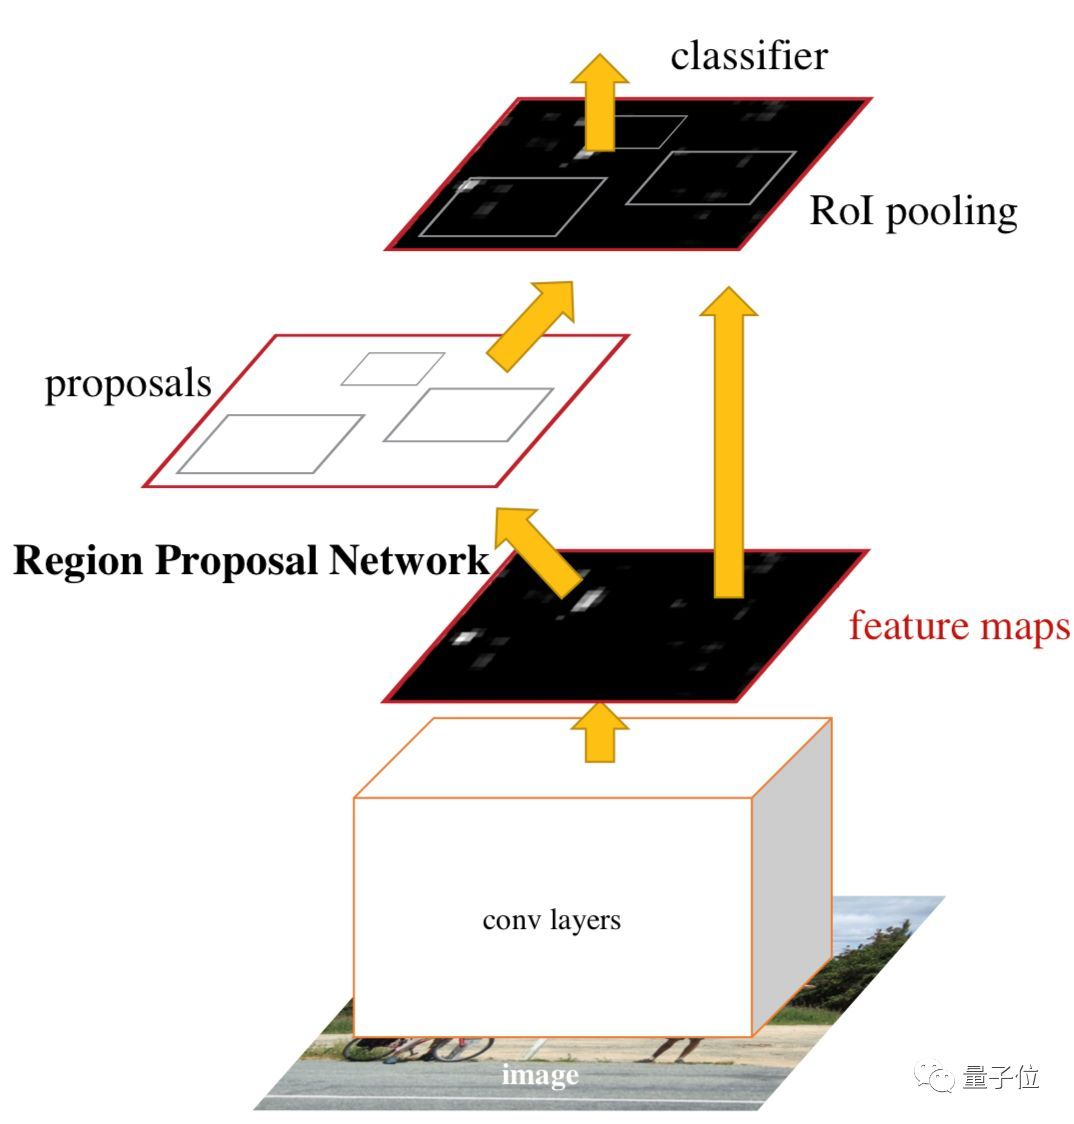
\includegraphics[width=0.4\textwidth]{Segmentacion con redes neuronales/Faster R-CNN/esquema.jpeg}
	\caption[Esquema del funcionamiento de Faster R-CNN]{Esquema del funcionamiento de Faster R-CNN (Fuente: \url{https://medium.com/egen/region-proposal-network-rpn-backbone-of-faster-r-cnn-4a744a38d7f9})}
	\label{fig:Faster R-CNN esquema}
\end{figure}

Siguiendo con el objetivo de poder comparar redes neuronales y su evolución con el paso de los años, en esta sección se van a desarrollar dos redes tipo Faster R-CNN basadas en LEGONet y LEGO16.
\newpage
\subsection{Faster R-CNN basado en LEGONet}
LEGONet cuenta con un total de 25 capas, 5 son capas de convolución y 2 son completamente conectadas. En total cuenta con 60 millones de parámetros y 650.000 neuronas. Frente a los estándares actuales, es una red simple y fácil de entrenar pero antes es necesario modificar la para transformarla en una red tipo Faster R-CNN. En comparación con R-CNN, la transformación a Faster R-CNN es más laboriosa y requiere de más pasos.

\subsubsection*{Estructura}
\label{subsubsec: Faster R-CNN estructura}
El primer paso, es idéntico a R-CNN. Como se desea reentrenar LEGONet para detectar nuevos objetos, es necesario eliminar las tres últimas capas y sustituirlas por similares, pero con la dimensión correcta, que es el número total de clases que se desean detectar más un clase para el fondo.

\begin{itemize}
\item Capa 23: Completamente conectada (1x1x7) $\rightarrow$ (1x1x4)
\item Capa 24: \textit{Softmax} (1x1x1000) $\rightarrow$ (1x1x4)
\item Capa 23: Salida del clasificador
\end{itemize}

Una vez se ha terminado de modificar las capas centradas en clasificación, es el momento de añadir a la red neuronal el sistema encargado de determinar las posibles regiones de interés. Tal y como se ha explicado en la introducción a Faster R-CNN, dentro de la red neuronal, hay una sección dedicada al cálculo de posibles regiones de interés y ello a través de capas de convolución. El primer paso para la creación de esta sección es la determinación de la capa para la extracción de características. En este caso, como se trabaja con una variante de AlexNet, la capa escogida es Relu5. Se trata de una capa del tipo \textit{Max pooling} que será sustituida par una del tipo ROI \textit{Max pooling}. Las capas \textit{Max pooling} se encargan de reducir las dimensiones de las capas internas de una red para evitar que estas crezcan demasiado, en comparación, \textit{ROI Max pooling} cumple una función similar pero con la diferencia de ser capaz de ajustarse para trabajar con dimensiones no uniformes.

Tras estos cambios, la red ya esta preparada para introducir dentro de esta misma a una red encargada de proponer regiones de interés (Region Proposal Network - RPN). Esta nueva red RPN se caracteriza porque internamente esta constituida por capas de convolución y una capa de clasificación. Este clasificador determina la probabilidad de que las regiones de interés tengan un objeto. Toda esta información extraída se manda a la capa de \textit{ROI Max pooling} para así poder analizar la imagen por completo y determinar la presencia de objetos en la imagen. Para que esto funcione correctamente y se pueda entrenar a la red, es necesario incluir dos capas más al final de la red para ayudar a determinar las regiones de interés. Estas últimas capas son una capa completamente conectada y una capa \textit{Box regression}. Tras aplicar todos los cambios mencionados, la estructura final de la red se puede observar en la \autoref{fig:Faster R-CNN LEGONet arquitectura}.

\begin{figure}[ht]  %Esquema Faster R-CNN RPN
	\centering
	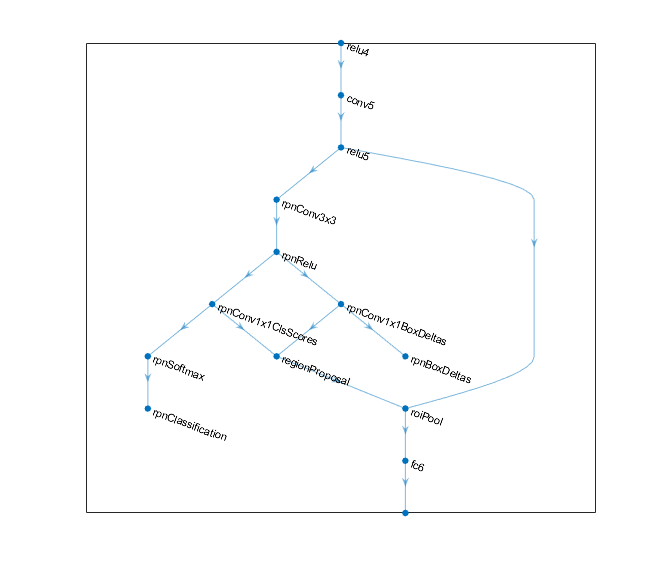
\includegraphics[width=0.6\textwidth]{Segmentacion con redes neuronales/Faster R-CNN/RPN LEGONet.png}
	\caption{Esquema de la red RPN empleada en Faster R-CNN basado en LEGONet}
	\label{fig:Faster R-CNN RPN}
\end{figure}

\begin{figure}[ht]  %Estructura Faster R-CNN
	\centering
	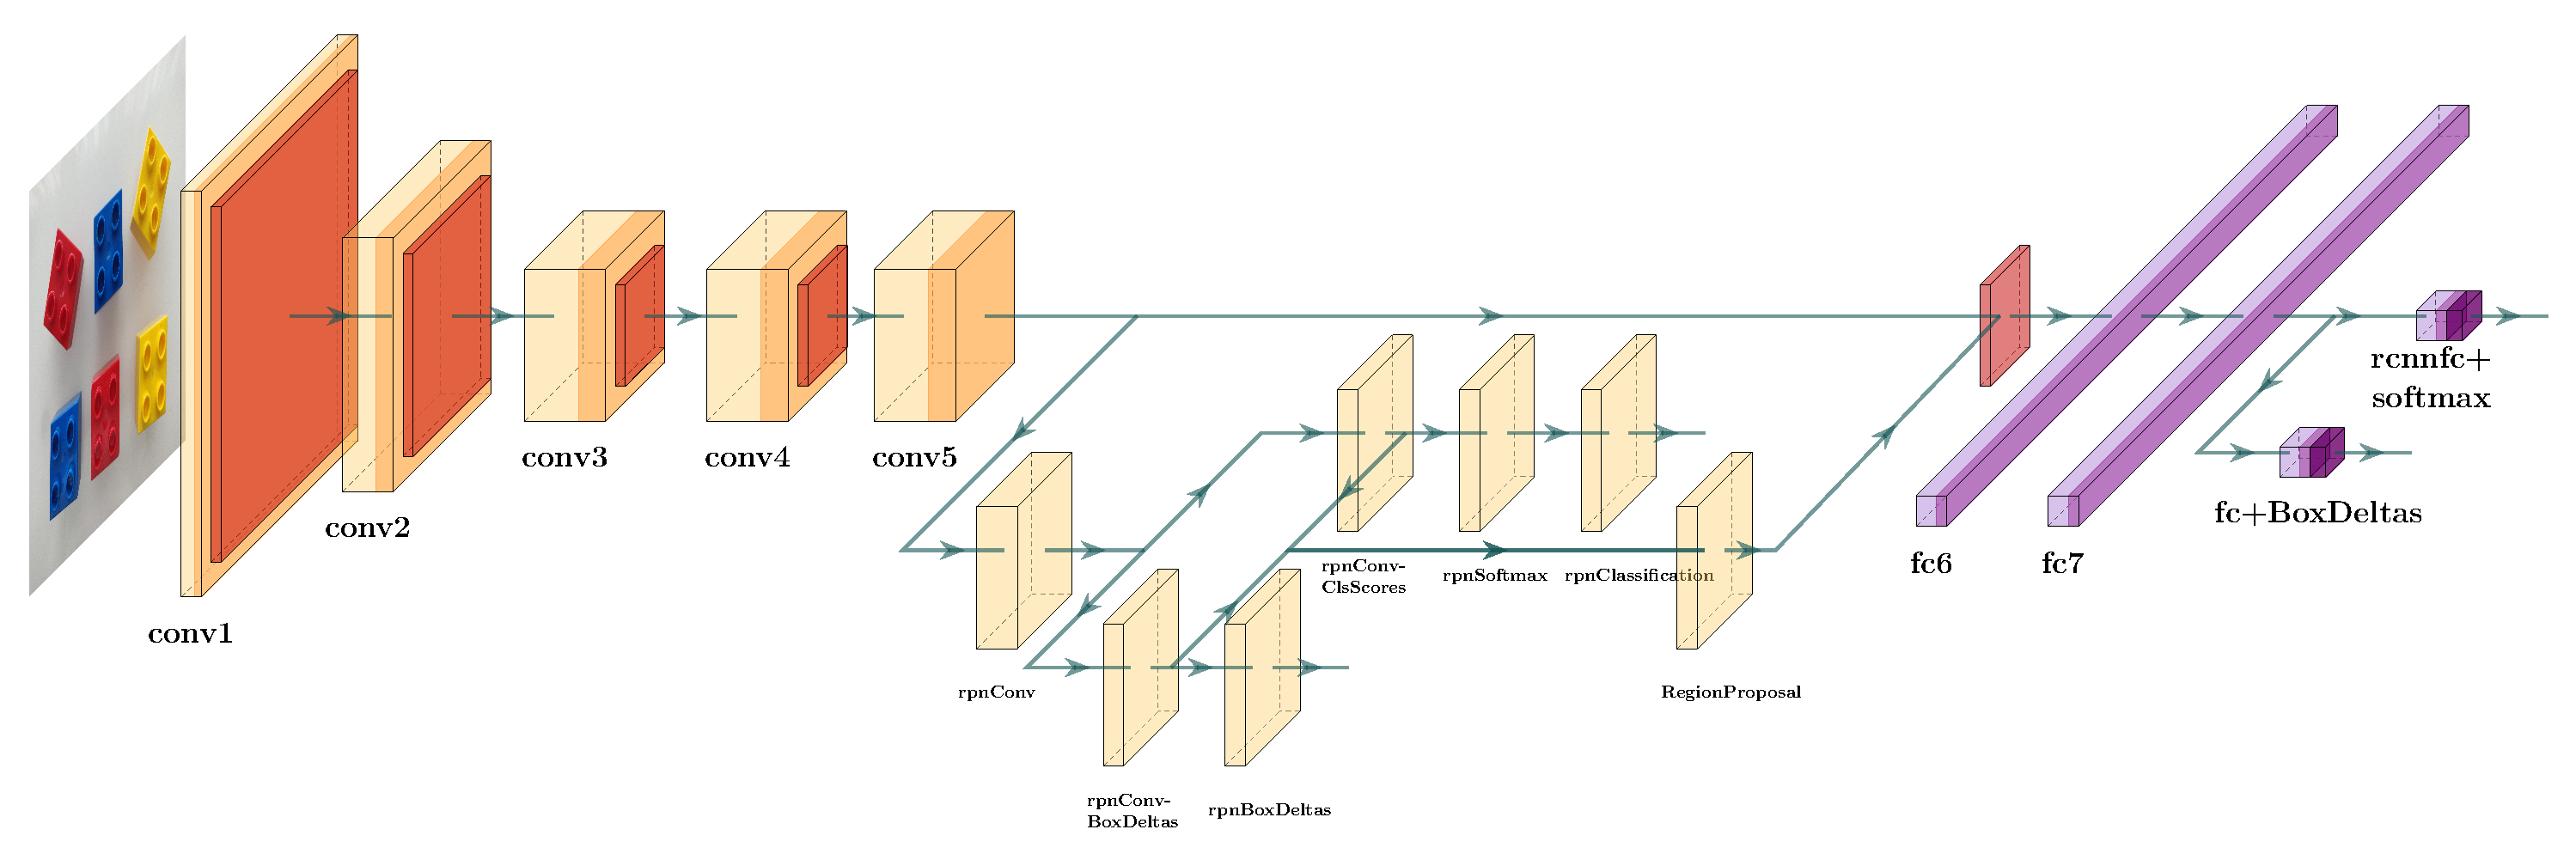
\includegraphics[width=1\textwidth]{Segmentacion con redes neuronales/Faster R-CNN/Faster_RCNN_LEGONet.pdf}
	\caption{Estructura de Faster R-CNN basado en LEGONet}
	\label{fig:Faster R-CNN LEGONet arquitectura}
\end{figure}


\subsubsection*{Entrenamiento}
Para el entrenamiento de esta red se ha usado la base de datos diseñada en la \autoref{sec:Preparativos para el de entrenamiento detectores}. Esta base de datos consta de un total de 2.076 imágenes con un total de 5.886 piezas de LEGO. Se han realizado numerosas pruebas de entrenamiento y tras numerosas pruebas se ha descubierto que la red presentaba problemas para aprender debido a la red RPN, esta tardaba en aprender y por ello evitaba que el clasificador también aprendiese. Por ello, el aprendizaje se ha realizado en cuatro etapas muy parecidas pero con el objetivo de ir enseñando poco a poco al clasificador y a la red RPN. En el caso de Faster R-CNN el sistema depende de la red RPN para poder entrenar y esta a su vez depende del clasificador ya que extrae información con sus capas de convolución. Es por ello por lo que el proceso de aprendizaje es del tipo iterativo. La red se ha entrenado cuatro veces de forma que en cada etapa la red RPN pueda ser reentrenada con los nuevos pesos de las capas de convolución. Tras varias pruebas, se ha determinado que las mejores opciones para el entrenamiento son las mostradas en la \autoref{tab:Faster RCNN LEGONet options}.

\begin{table}[ht]
  \centering
    \begin{tabular}{|l|c|}
    \hline
    \multicolumn{2}{|c|}{Opciones de entrenamineto} \\
    \hline
    Solver & \multicolumn{1}{l|}{Stochastic Gradient Descent with Momentum (SGDM)} \\
    \hline
    Momentum & 0.9 \\
    \hline
    Initial Learn Rate & 1.00E-04 \\
    \hline
    Learn Rate Schedule & piecewise \\
    \hline
    Learn Rate Drop Factor & 0.1 \\
    \hline
    Learn Rate Drop Period & 70 \\
    \hline
    L2Regularization & 0.004 \\
    \hline
    Max Epochs & 100-100-100-100 \\
    \hline
    Mini Batch Size & 200 \\
    \hline
    Shuffle data & every epoch \\
    \hline
    \end{tabular}%
  \caption{Opciones de entrenamiento de Faster R-CNN basado en LEGONet}
  \label{tab:Faster RCNN LEGONet options}%
\end{table}%


\subsubsection*{Resultados}
Con la ayuda del \textit{script} definido en la \autoref{subsec:evaluacion}, se han podido obtener cuatro parámetros que permiten evaluar la capacidad de esta red: tasa de fallos, falsos positivos por imagen (FPPI), precisión de los \textit{bounding boxes} y la exhaustividad. Al correr un detector de objetos existen múltiples parámetros a definir por el usuario que marcan el comportamiento de la red. Se ha evaluado la red con todas las posibles combinaciones de parámetros lógicas y se ha determinado el mejor rango de funcionamiento de la red. Estos parámetros son el nivel de superposición de las \textit{bounding boxes} y el límite de incertidumbre aceptable para determinar que lo detectado es un objeto. Al analizar todos los casos lógicos se han obtenido los resultados mostrados en la \autoref{fig:Faster RCNN LEGONet evaluacion}. En el eje x se puede ver los casos que se han analizado. El umbral de confianza se ha variado desde 0.5 hasta 1 en intervalos de 0.05 y para cada caso se ha evaluado modificando el nivel de superposición entre \textit{bounding boxes}. El nivel de superposición se ha variado entre 0 y 0.5 con intervalos de 0.05.

\begin{figure}[ht]  %Evaluación de Faster R-CNN basado en LEGONet
	\centering
	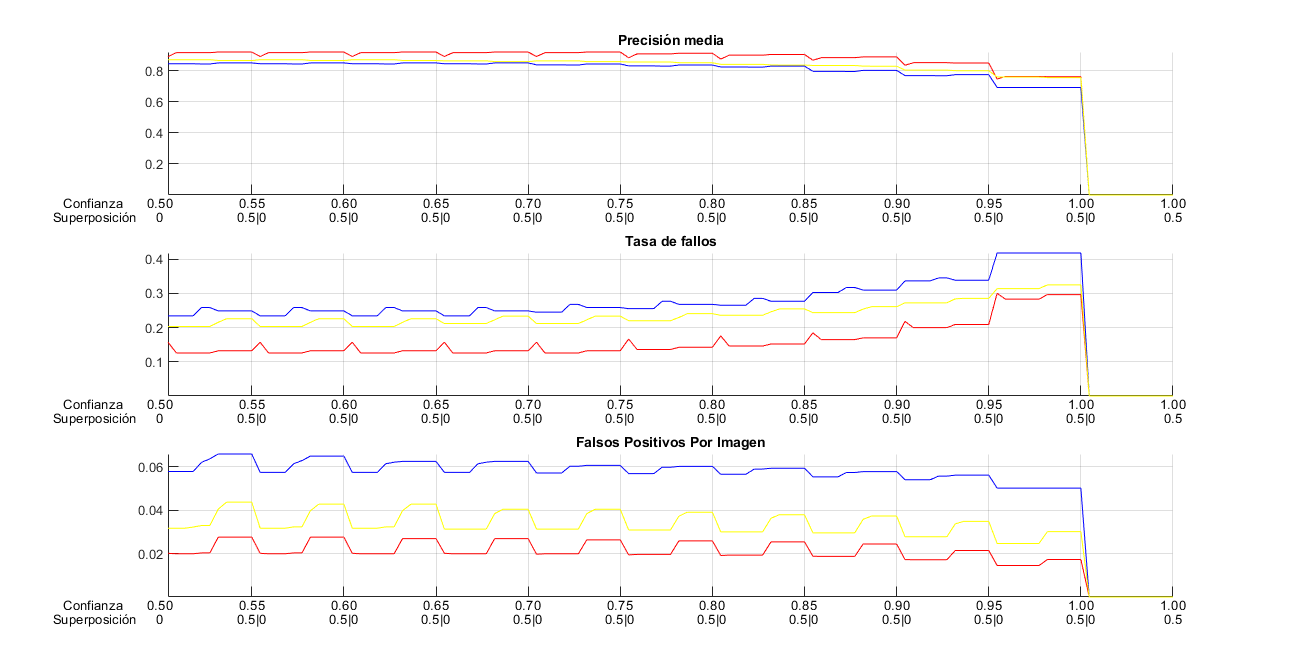
\includegraphics[width=1\textwidth]{Segmentacion con redes neuronales/Faster R-CNN/evaluacion legonet.png}
	\caption{Evaluación de Faster R-CNN basado en LEGONet en función de diversos parámetros}
	\label{fig:Faster RCNN LEGONet evaluacion}
\end{figure}


Analizando estos resultados, se ha determinado que un buen punto de compromiso entre precisión, tasa de fallos y falsos positivos se obtiene con un límite de incertidumbre de 0.65 y un factor de superposición de 0.05. En los resultados mostrados a continuación se ha trabajado en este punto de operación. Tras analizar observamos que todas las gráficas presentan peores resultados frente a R-CNN. Esto es algo de esperar ya que Faster R-CNN reduce precisión a cambio de rapidez. Aun así, los resultados son positivos y demuestra que la red ha aprendido.

\begin{itemize}
\item Amarillo: El error cometido al detectar las piezas tanto en precisión como en fallos y falsos positivos en demasiado elevado como para poder ser implantado. Además se observa que el exhaustividad nunca llega a uno lo cual es debido a la presencia de falsos positivos. También se observa como la precisión es demasiado baja como para ser implantado.
\item Rojo: El rojo presenta una situación similar al amarillo, aunque con un menor número de falsos positivos. Presenta una tasa de fallos y una precisión un poco baja como para poder ser implantada.
\item Azul: El azul se asemeja bastante al amarillo en la distribución de sus gráficas, aunque en general ha obtenido mejores resultados.
\end{itemize}

Analizando los resultados en conjunto se puede ver que la red ha tenido problemas para distinguir las piezas. Aunque se esperaba unos resultados inferiores a la red R-CNN basado en LEGONet estos son más bajos a lo esperado. Sería recomendable dedicar más tiempo al entrenamiento de esta red y con mayor potencia para así poder comprobar la verdadera capacidad de esta red. Se puede observar una mejor comparación entre todos los métodos en el \autoref{chap:Resultados}.

\begin{figure}[ht]  %Estudio Amarillo
  \subfloat{
	\begin{minipage}[c][1\width]{0.49\textwidth}
	   \centering
	   \includegraphics[width=1\textwidth]{Segmentacion con redes neuronales/Faster R-CNN/precision yellow legonet.png}
	\end{minipage}}
  \hfill	
  \subfloat{
	\begin{minipage}[c][1\width]{0.49\textwidth}
	   \centering
	   \includegraphics[width=1\textwidth]{Segmentacion con redes neuronales/Faster R-CNN/miss yellow legonet.png}
	\end{minipage}}
\caption{Estudio de la segmentación por Faster R-CNN basado en LEGONet al detectar piezas amarillas}
\label{fig:yellow Faster R-CNN LEGONet}
\vspace{-5pt}
\end{figure}

\begin{figure}[ht]  %Estudio Rojo
  \subfloat{
	\begin{minipage}[c][1\width]{0.49\textwidth}
	   \centering
	   \includegraphics[width=1\textwidth]{Segmentacion con redes neuronales/Faster R-CNN/precision red legonet.png}
	\end{minipage}}
  \hfill	
  \subfloat{
	\begin{minipage}[c][1\width]{0.49\textwidth}
	   \centering
	   \includegraphics[width=1\textwidth]{Segmentacion con redes neuronales/Faster R-CNN/miss red legonet.png}
	\end{minipage}}
\caption{Estudio de la segmentación por Faster R-CNN basado en LEGONet al detectar piezas rojas}
\label{fig:red Faster R-CNN LEGONet}
\vspace{-5pt}
\end{figure}

\begin{figure}[ht]  %Estudio Azul
  \subfloat{
	\begin{minipage}[c][1\width]{0.49\textwidth}
	   \centering
	   \includegraphics[width=1\textwidth]{Segmentacion con redes neuronales/Faster R-CNN/precision blue legonet.png}
	\end{minipage}}
  \hfill	
  \subfloat{
	\begin{minipage}[c][1\width]{0.49\textwidth}
	   \centering
	   \includegraphics[width=1\textwidth]{Segmentacion con redes neuronales/Faster R-CNN/miss blue legonet.png}
	\end{minipage}}
\caption{Estudio de la segmentación por Faster R-CNN basado en LEGONet al detectar piezas azules}
\label{fig:blue Faster R-CNN LEGONet}
\vspace{-5pt}
\end{figure}


\newpage
\subsection{Faster R-CNN basasdo en LEGO16}
LEGO16 cuenta con un total de 41 capas, 13 son capas de convolución y 3 son completamente conectadas. En total cuenta con 138 millones de parámetros y 13 millones de neuronas. Frente a LEGONet, se trata de una red grande y pesada que requiere de más tiempo y potencia para ser entrenada, pero antes es necesario modificar la para transformarla en una red tipo Faster R-CNN. En comparación con R-CNN, la transformación a Faster R-CNN es más laboriosa y requiere de más pasos.

\subsubsection*{Estructura}
El proceso para la obtención de una red tipo Faster R-CNN basado en LEGO16 es muy similar al proceso basado en LEGONet. En ambos casos se comienza por la variación del clasificador para la detección de las nuevas clases y a continuación se añade la red RPN para la detección de regiones de interés. La principal diferencia reside en como se implanta la red RPN dentro del clasificador, como ya se ha visto en la \autoref{subsubsec: Faster R-CNN estructura}, en LEGONet se introdujo en la capa ReLu5. En el caso de LEGO16, como se desea que las capas de convolución extraigan toda la información posible, la red RPN se implanta en la capa ReLu5\_3 tras las últimas capas de convolución. Tras aplicar todos los cambios se obtiene la estructura final de la red, esta se muestra en la \autoref{fig:Faster R-CNN LEGO16 arquitectura}.


\begin{figure}[ht]  %Esquema Faster R-CNN RPN
	\centering
	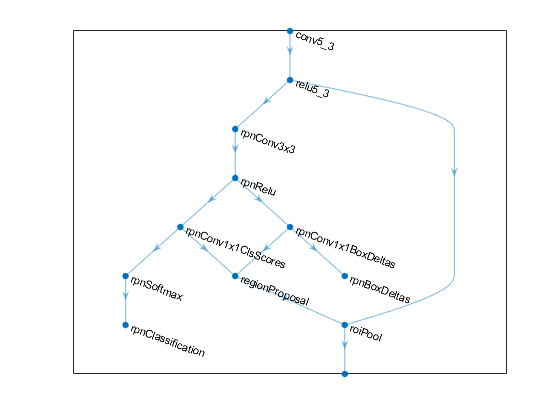
\includegraphics[width=0.6\textwidth]{Segmentacion con redes neuronales/Faster R-CNN/RPN LEGO16.png}
	\caption{Esquema de la red RPN empleada en Faster R-CNN basado en LEGO16}
	\label{fig:Faster R-CNN RPN LEGO16}
\end{figure}

\begin{figure}[ht]  %Esquema Faster R-CNN basado en LEGO16
	\centering
	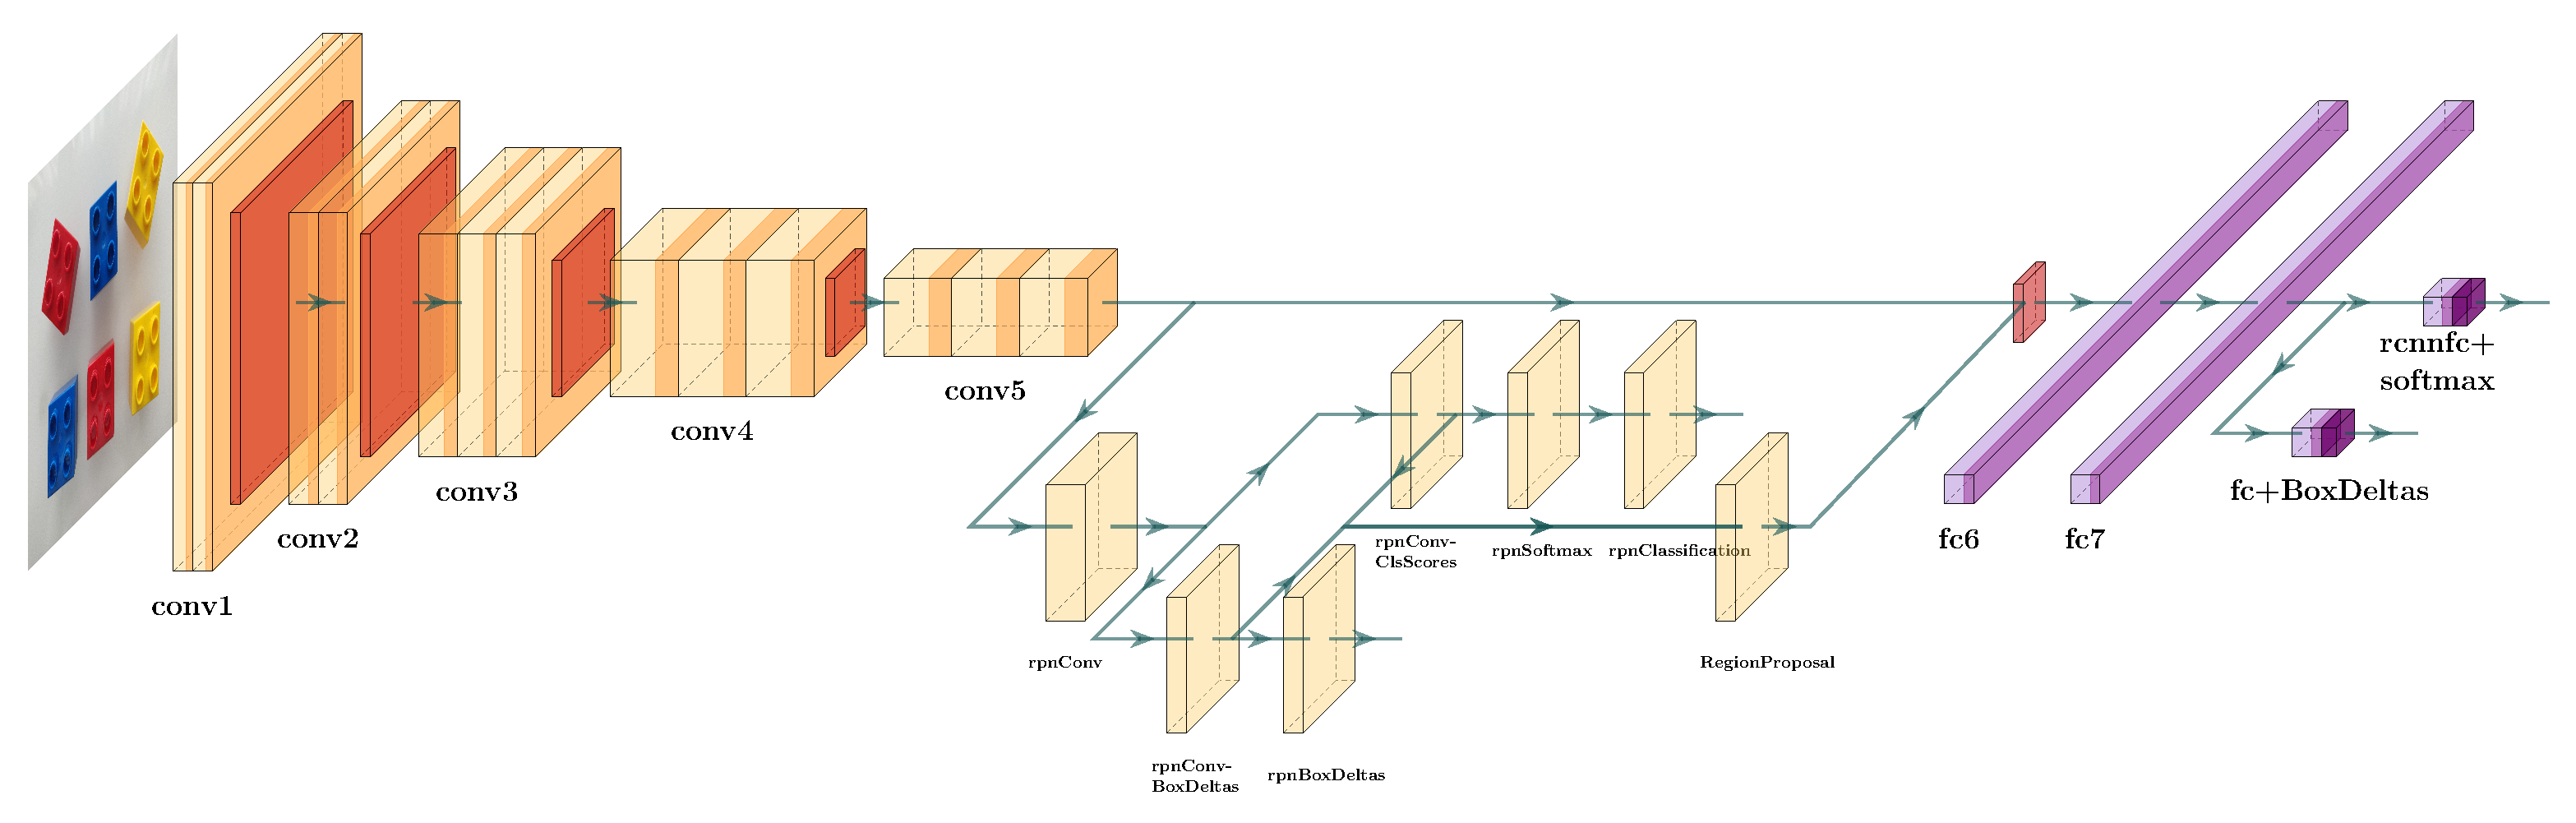
\includegraphics[width=1\textwidth]{Segmentacion con redes neuronales/Faster R-CNN/Faster_RCNN_LEGO16.pdf}
	\caption{Estructura de Faster R-CNN basado en LEGO16}
	\label{fig:Faster R-CNN LEGO16 arquitectura}
\end{figure}

\subsubsection*{Entrenamiento}
Para el entrenamiento de esta red se ha usado la base de datos diseñada en la \autoref{sec:Preparativos para el de entrenamiento detectores}. Esta base de datos consta de un total de 2.076 imágenes con un total de 5.886 piezas de LEGO. Se han realizado numerosas pruebas de entrenamiento y tras numerosas pruebas se ha descubierto que la red presentaba problemas para aprender debido a la red RPN, esta tardaba en aprender y por ello evitaba que el clasificador también aprendiese. Por ello, el aprendizaje se ha realizado en cuatro etapas muy parecidas pero con el objetivo de ir enseñando poco a poco al clasificador y a la red RPN. En el caso de Faster R-CNN el sistema depende de la red RPN para poder entrenar y esta a su vez depende del clasificador ya que extrae información con sus capas de convolución. Es por ello por lo que el proceso de aprendizaje es del tipo iterativo. La red se ha entrenado cuatro veces de forma que en cada etapa la red RPN pueda ser reentrenada con los nuevos pesos de las capas de convolución. Tras varias pruebas, se ha determinado que las mejores opciones para el entrenamiento son las mostradas en la \autoref{tab:Faster RCNN LEGO16 options}.

\begin{table}[ht]
  \centering
    \begin{tabular}{|l|c|}
    \hline
    \multicolumn{2}{|c|}{Opciones de entrenamineto} \\
    \hline
    Optimizador & \multicolumn{1}{l|}{Stochastic Gradient Descent with Momentum (SGDM)} \\
    \hline
    Momentum & 0.9 \\
    \hline
    Initial Learn Rate & 1.00E-03 \\
    \hline
    Learn Rate Schedule & piecewise \\
    \hline
    Learn Rate Drop Factor & 0.1 \\
    \hline
    Learn Rate Drop Period & 70 \\
    \hline
    L2Regularization & 0.004 \\
    \hline
    Max Epochs & 30-30-30-30 \\
    \hline
    Mini Batch Size & 3 \\
    \hline
    Shuffle data & every epoch \\
    \hline
    \end{tabular}%
  \caption{Opciones de entrenamiento de Faster R-CNN basado en LEGO16}
  \label{tab:Faster RCNN LEGO16 options}%
\end{table}%

\subsubsection*{Resultados}
Con la ayuda del \textit{script} definido en la \autoref{subsec:evaluacion}, se han podido obtener cuatro parámetros que permiten evaluar la capacidad de esta red: tasa de fallos, falsos positivos por imagen (FPPI), precisión de los \textit{bounding boxes} y la exhaustividad. Al correr un detector de objetos existen múltiples parámetros a definir por el usuario que marcan el comportamiento de la red. Se ha evaluado la red con todas las posibles combinaciones de parámetros lógicas y se ha determinado el mejor rango de funcionamiento de la red. Estos parámetros son el nivel de superposición de las \textit{bounding boxes} y el límite de incertidumbre aceptable para determinar que lo detectado es un objeto. Al analizar todos los casos lógicos se han obtenido los resultados mostrados en la \autoref{fig:Faster RCNN LEGO16 evaluacion}. En el eje x se puede ver los casos que se han analizado. El umbral de confianza se ha variado desde 0.5 hasta 1 en intervalos de 0.05 y para cada caso se ha evaluado modificando el nivel de superposición entre \textit{bounding boxes}. El nivel de superposición se ha variado entre 0 y 0.5 con intervalos de 0.05.

\begin{figure}[ht]  %Evaluación de Faster R-CNN basado en LEGO16
	\centering
	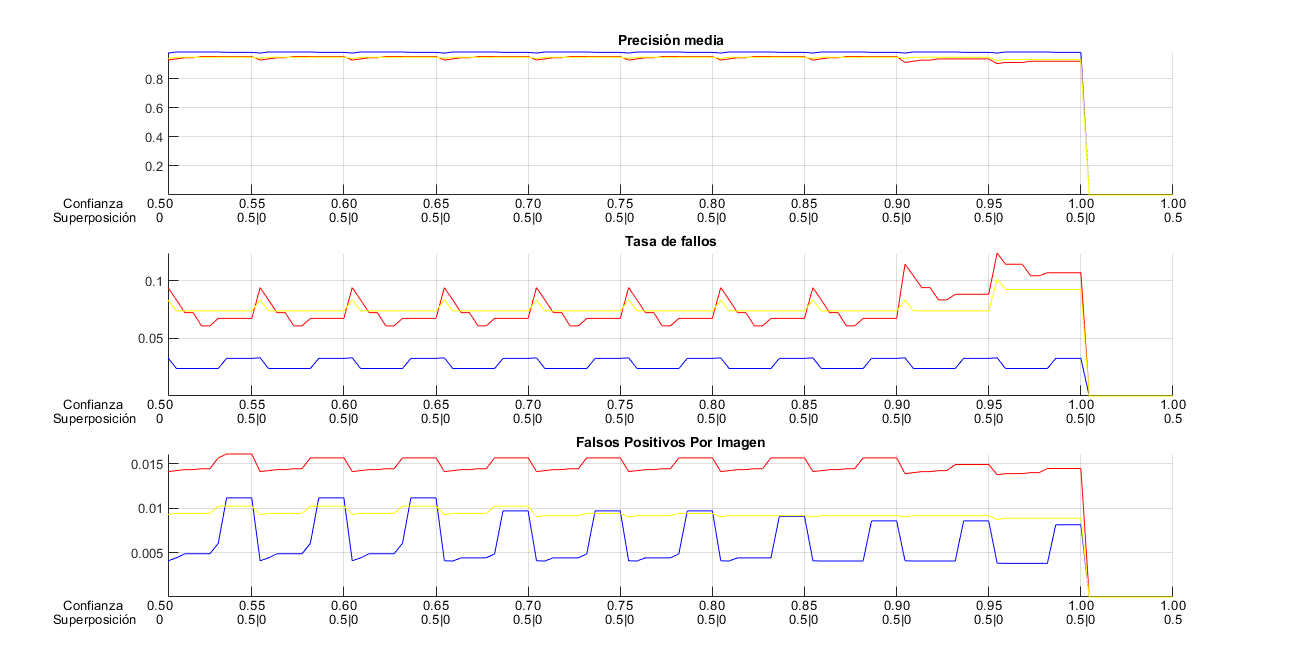
\includegraphics[width=1\textwidth]{Segmentacion con redes neuronales/Faster R-CNN/evaluacion lego16.png}
	\caption{Evaluación de Faster R-CNN basado en LEGO16 en función de diversos parámetros}
	\label{fig:Faster RCNN LEGO16 evaluacion}
\end{figure}

Analizando estos resultados, se ha determinado que un buen punto de compromiso entre precisión, tasa de fallos y falsos positivos se obtiene con un límite de incertidumbre de 0.85 y un factor de superposición de 0.20. En los resultados mostrados a continuación se ha trabajado en este punto de operación. Tras analizar observamos que todas las gráficas presentan mejores resultados frente a Faster R-CNN basado en LEGONet. Esto es algo de esperar ya que LEGO16 es una red mayor, más compleja y con más capacidad para extraer características.

\begin{itemize}
\item Amarillo: La tasa de fallos es demasiado elevado en comparación al resto de resultados y similar al obtenido con la segmentación por color en el \autoref{chap:Segmentacion con mascaras de color}. Por el contrario, los falsos positivos por imagen son bastante reducidos en general y la precisión es bastante elevada.
\item Rojo: El rojo se asemeja bastante al amarillo tanto en precisión como tasa de fallos y falsos positivos.
\item Azul: El azul presenta los mejores resultados de los tres. La precisión es muy elevada y la tasa de fallos son muy bajos, aunque los falsos positivos son superiores al rojo y amarillo.
\end{itemize}

Analizando los resultados en conjunto se puede ver que la red no ha tenido problemas para distinguir las piezas. Se esperaba unos resultados superiores a los de Faster R-CNN basado en LEGONEt y ha cumplido con las expectativas aunque sería recomendable dedicar más tiempo al entrenamiento de esta red y con mayor potencia para así poder comprobar la verdadera capacidad de esta red. Se puede observar una mejor comparación entre todos los métodos en el \autoref{chap:Resultados}.

\begin{figure}[ht]  %Estudio Amarillo
  \subfloat{
	\begin{minipage}[c][1\width]{0.49\textwidth}
	   \centering
	   \includegraphics[width=1\textwidth]{Segmentacion con redes neuronales/Faster R-CNN/precision yellow lego16.png}
	\end{minipage}}
  \hfill	
  \subfloat{
	\begin{minipage}[c][1\width]{0.49\textwidth}
	   \centering
	   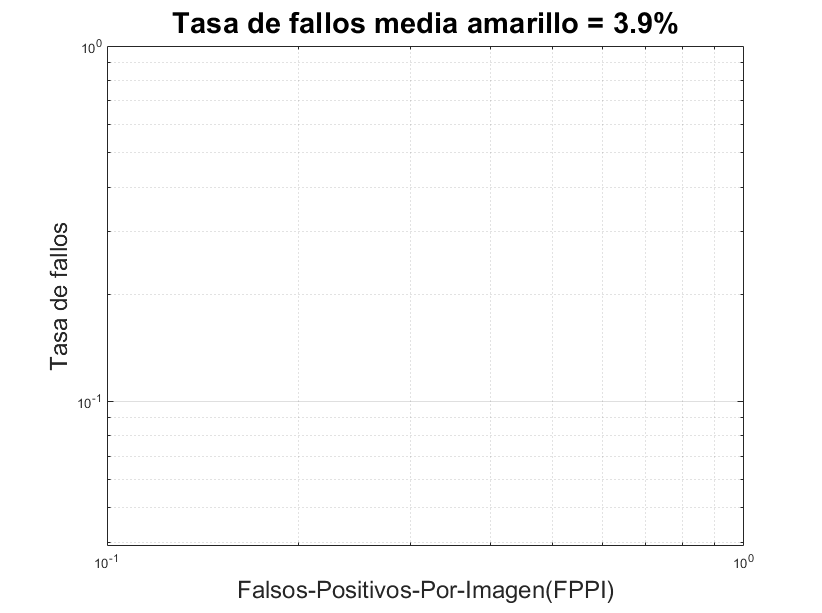
\includegraphics[width=1\textwidth]{Segmentacion con redes neuronales/Faster R-CNN/miss yellow lego16.png}
	\end{minipage}}
\vspace{-5pt}
\caption{Estudio de la segmentación por Faster R-CNN basado en LEGO16 al detectar piezas amarillas}
\label{fig:yellow Faster R-CNN LEGO16}
\end{figure}

\begin{figure}[ht]  %Estudio Rojo
  \subfloat{
	\begin{minipage}[c][1\width]{0.49\textwidth}
	   \centering
	   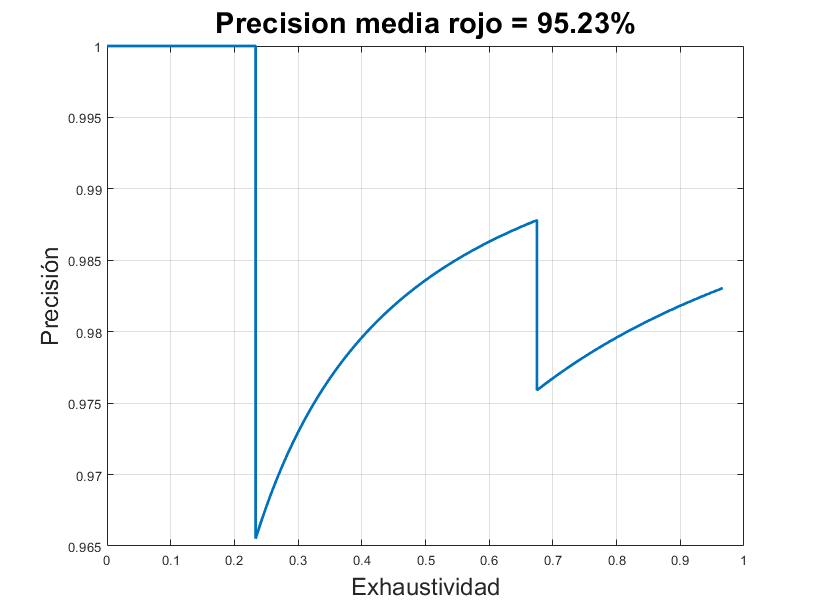
\includegraphics[width=1\textwidth]{Segmentacion con redes neuronales/Faster R-CNN/precision red lego16.png}
	\end{minipage}}
  \hfill	
  \subfloat{
	\begin{minipage}[c][1\width]{0.49\textwidth}
	   \centering
	   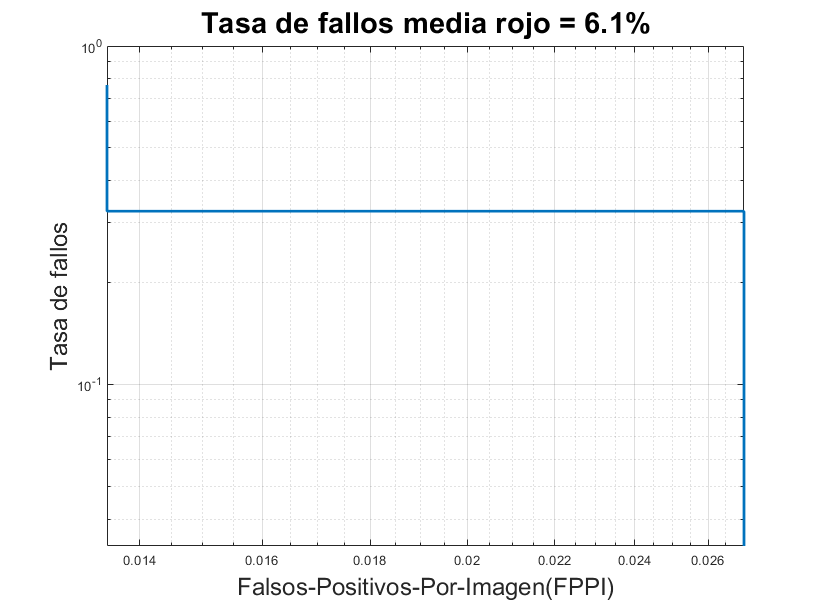
\includegraphics[width=1\textwidth]{Segmentacion con redes neuronales/Faster R-CNN/miss red lego16.png}
	\end{minipage}}
\vspace{-5pt}
\caption{Estudio de la segmentación por Faster R-CNN basado en LEGO16 al detectar piezas rojas}
\label{fig:red Faster R-CNN LEGO16}
\end{figure}

\begin{figure}[ht]  %Estudio Azul
  \subfloat{
	\begin{minipage}[c][1\width]{0.49\textwidth}
	   \centering
	   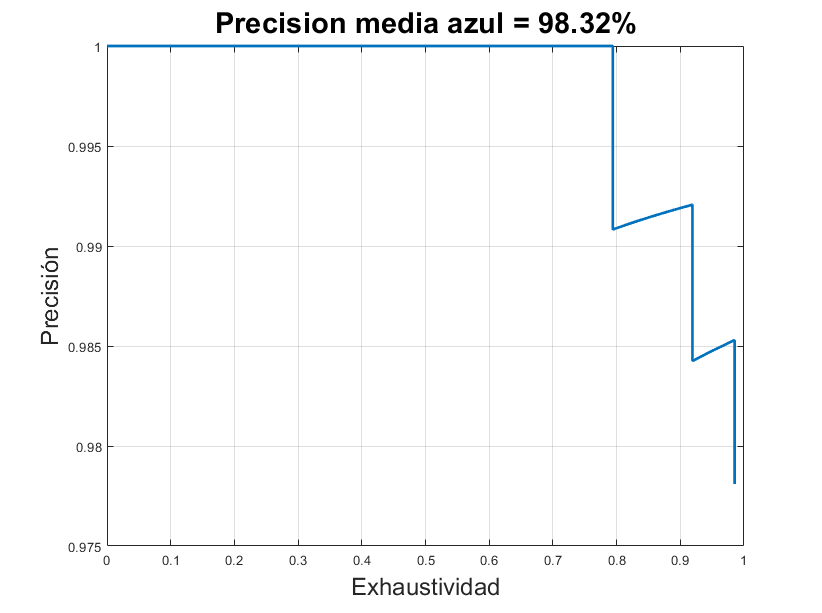
\includegraphics[width=1\textwidth]{Segmentacion con redes neuronales/Faster R-CNN/precision blue lego16.png}
	\end{minipage}}
  \hfill	
  \subfloat{
	\begin{minipage}[c][1\width]{0.49\textwidth}
	   \centering
	   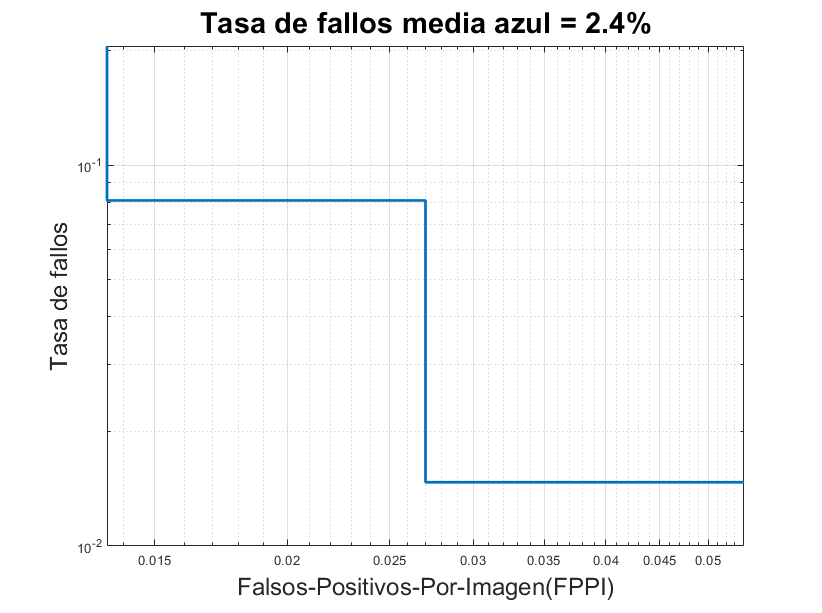
\includegraphics[width=1\textwidth]{Segmentacion con redes neuronales/Faster R-CNN/miss blue lego16.png}
	\end{minipage}}
\vspace{-5pt}
\caption{Estudio de la segmentación por Faster R-CNN basado en LEGO16 al detectar piezas azules}
\label{fig:blue Faster R-CNN LEGO16}
\end{figure}


%%%%%%%%%%%%%%%%%%%%%%%%%%%%%%%%%%%%%%%%%%%%%%%%%%%%%%%%%%%%%%%%%%%%%%%%%%%%%%%%%%%%%%%%%%%%%%%%%%%%%%%%%%%%%
%%%%%%%%%%%%%%%%%%%%%%%%%%%%%%%%%%%%%%%%%%%%%%%%%%%%%%%%%%%%%%%%%%%%%%%%%%%%%%%%%%%%%%%%%%%%%%%%%%%%%%%%%%%%%
\newpage
\section{YOLO}
En 2015 se produjo una revolución que cambió la forma de trabajar con las redes neuronales y nuestro entendimiento de estas. En 2015 cuatro investigadores de la universidad de Washington desarrollaron un nuevo tipo de red neuronal bautizada como YOLO (You Only Look Once) \citep{YOLO}. Esta nueva red se caracteriza porque tal y como su nombre indica, la imagen solo se ve una vez. Esto puede parecer similar a Faster R-CNN pero difiere bastante. En Faster R-CNN ya la imagen es primero pasada por las capas de convolución para a continuación determinar regiones de interés con la ayuda de una red tipo RPN y a continuación se analiza cada una de las posibles regiones de interés. Esto implica qué aunque inicialmente la imagen pase completamente por las capas de convolución, después se analiza por secciones por lo tanto es necesario analizar la misma imagen varias veces. Sin embargo, esto no sucede en YOLO por la forma interna en la que trabaja.

A diferencia de las redes ya vistas en este proyecto, YOLO no fue diseñada con la idea de reaprovechar un clasificador ya existente para detectar objetos. Se construyo desde cero y con el único objetivo de detectar objetos. Es decir, para detectar objetos no recurre a la técnica de correr un clasificador por diferentes regiones de la imagen y así detectar un objeto. YOLO emplea un método completamente diferente, este comienza por la división de la imagen en secciones, en el artículo original, se divide la imagen en una 7x7 secciones, aunque el número de secciones se pueden modificar. Para cada una de las secciones una capa convolucional predice un número de posibles \textit{bounding boxes} (área de la imagen que puede contener un objeto) así como la posible clase de cada \textit{bounding box} y su probabilidad de ser ese objeto. Por último, se analizan en conjunto todos los \textit{bounding boxes} definidos así como su clase y su probabilidad y se determina cuáles son los objetos en la imagen y donde están. Este método presenta numerosas ventajas frente a R-CNN y Faster R-CNN, en primer lugar, destaca por su rapidez. La red diseñada por los desarrolladores de YOLO cuenta con con 24 capas de convolución y es capaz de correr a 45 imágenes por segundo. Esta red también se caracteriza por tener una estructura más propia de las Fully Convolutional Neuronal Network (FCNN), es decir, se caracteriza por ser mayoritariamente convolucional. Otra de sus grandes ventajas, es que al mirar a la imagen entera, es capaz de ver la diferentes conexiones entre \textit{bounding boxes} y determinar de forma rápida y precisa la posición del objeto. Esto no ocurre en métodos como la ventana flotante. A continuación, se muestra de forma breve y gráfica el funcionamiento de YOLO en la \autoref{fig:YOLO esquema}

Siguiendo con el objetivo de poder comparar redes neuronales y su evolución con el paso de los años, en esta sección se van a desarrollar dos redes tipo YOLO basadas en LEGONet y LEGO16. Debido al gran interés y las capacidades de YOLO, este ha sido desarrollado bastante en los últimos dos años. En la actualidad se han publicado cinco versiones de YOLO que mejoran su rendimiento y le dotan de más capacidades. Desgraciadamente, debido a la rapidez con la que se ha actualizado y desarrollado YOLO, en el momento de desarrollo de este proyecto MATLAB solo soporta hasta la segunda versión de YOLO. Es por ello que todas las redes del tipo YOLO se han basado en YOLO v2.

\begin{figure}[ht]  %Esquema Faster R-CNN
	\centering
	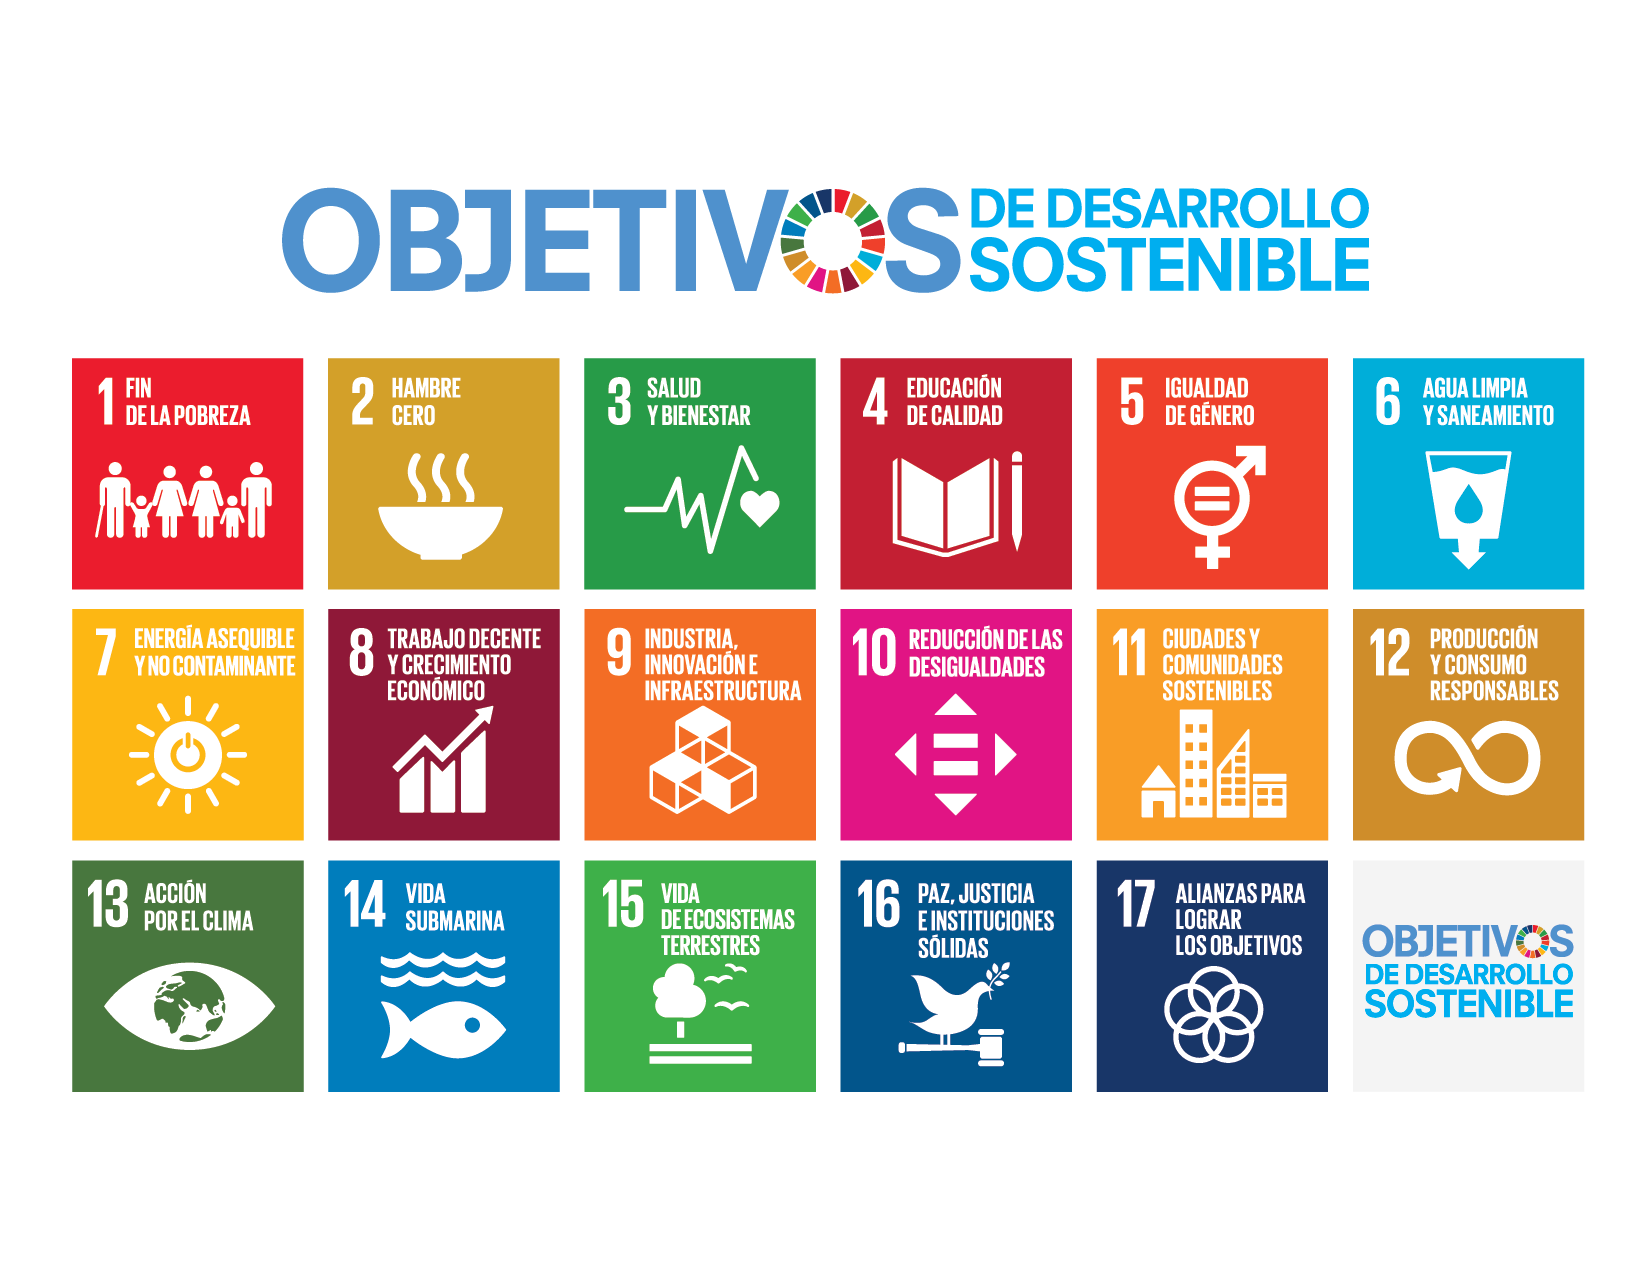
\includegraphics[width=0.8\textwidth]{Segmentacion con redes neuronales/YOLO/esquema.png}
	\caption[Esquema del funcionamiento de YOLO]{Esquema del funcionamiento de YOLO (Fuente: publiación original de YOLO \citep{YOLO})}
	\label{fig:YOLO esquema}
\end{figure}

\newpage
\subsection{YOLO basado en LEGONet}
LEGONet cuenta con un total de 25 capas, 5 son capas de convolución y 2 son completamente conectadas. En total cuenta con 60 millones de parámetros y 650.000 neuronas. Frente a los estándares actuales, es una red simple y fácil de entrenar, pero antes es necesario modificar la para transformarla en una red tipo YOLO.

\subsubsection*{Estructura}
YOLO se caracteriza por trabajar de forma diferente al resto de detectores de objetos ya que no se basa en un clasificador. Es por ello que aunque se vaya a partir de un clasificador, es necesario eliminar las últimas capas encargadas de la clasificación. El motivo por el que se parte de un clasificador es porque las primeras capas de convolución ya han sido entrenadas y se puede reaprovechar ese entrenamiento.

Con la ayuda de MATLAB, se han eliminado todas las capas de LEGONet pasado la capa Relu5 y se han sustituido por el sistema de YOLO. Esto implica la inclusión de dos capas de convolución acompañadas por capas \textit{Batch} y \textit{ReLu}. Y por último, se incluye una capa de transformación y la capa de salida. Estas dos últimas capas se encargan de coger las activaciones de las capas de convolución y redefinir los \textit{bounding boxes} para que se asemejen a los datos con los que han sido entrenados. Para que la red puede redefinir los \textit{bounding boxes}, necesita de una referencia. Al crear la red es necesario estipular el número de \textit{bounding boxes} y las dimensiones de los mismos que la red se puede encontrar y que empleará como referencia. En nuestro caso y con un par de pruebas, se ha encontrado que los mejores resultados se obtienen al definir un total de 5 posibles \textit{bounding boxes}.

\begin{figure}[ht]  %Estructura YOLO basado en LEGONet
	\centering
	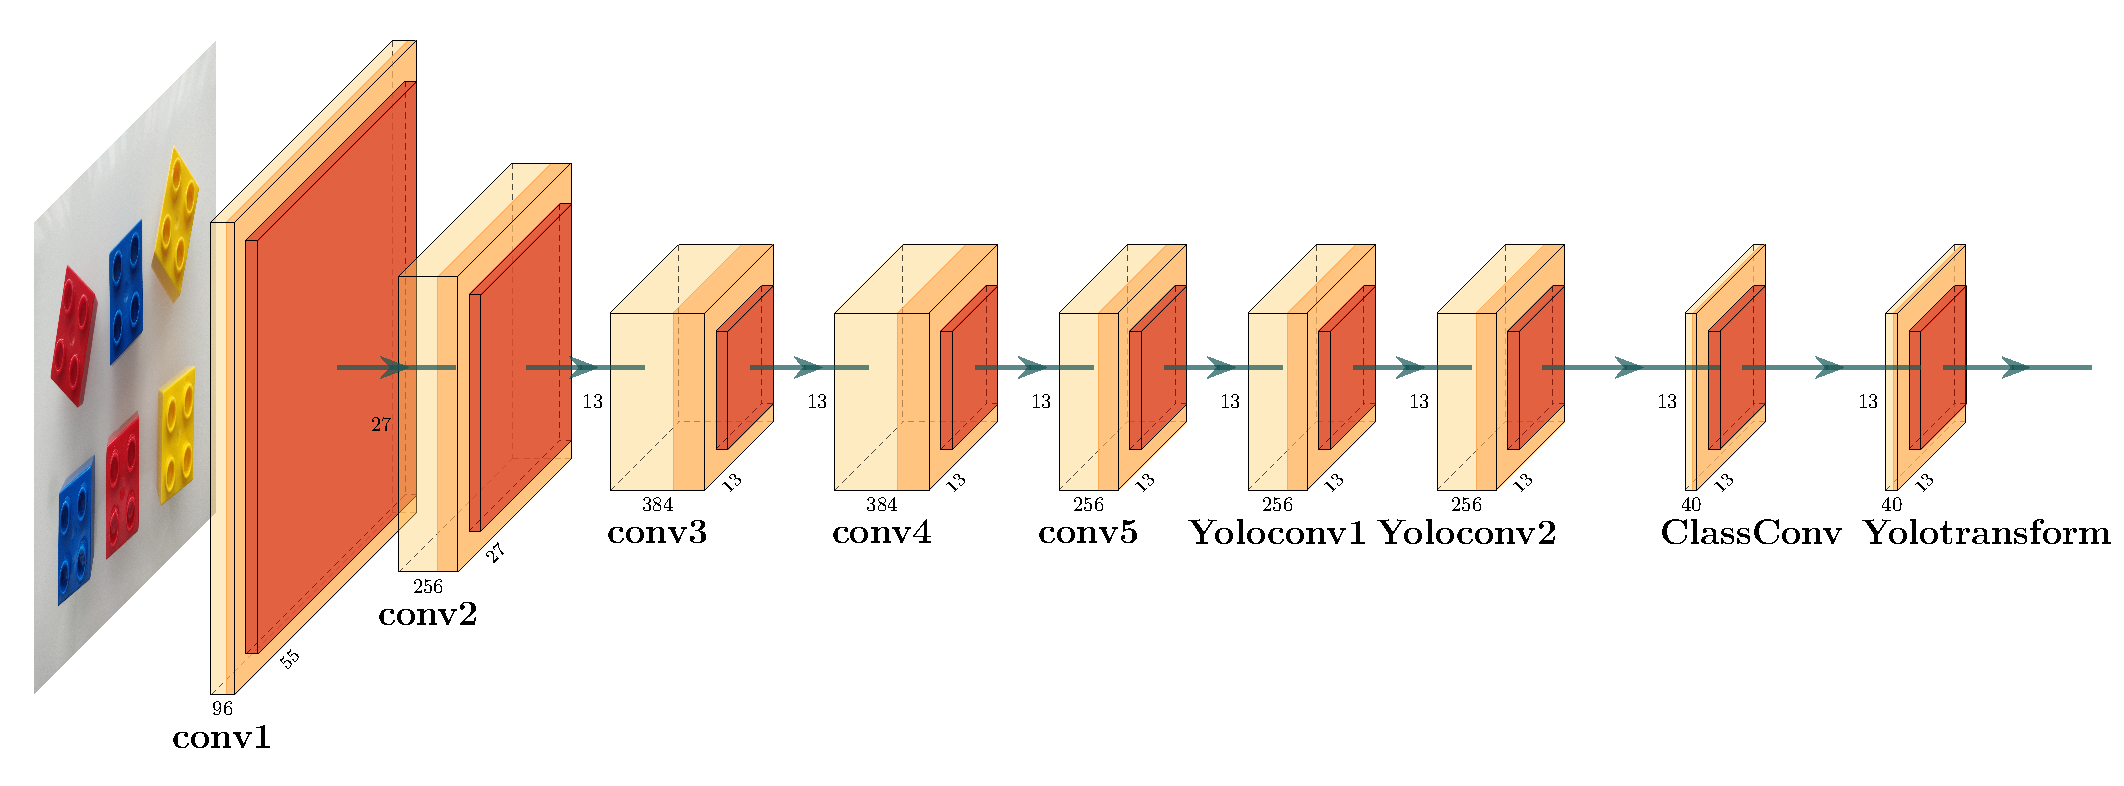
\includegraphics[width=0.8\textwidth]{Segmentacion con redes neuronales/YOLO/YOLO_LEGONet.pdf}
	\caption{Estructura de YOLO basado en LEGONet}
	\label{fig:YOLO LEGONet estructrua}
\end{figure}

\subsubsection*{Entrenamiento}
Para el entrenamiento de esta red se ha usado la base de datos diseñada en la \autoref{sec:Preparativos para el de entrenamiento detectores}. Esta base de datos consta de un total de 2.076 imágenes con un total de 5.886 piezas de LEGO. Se han realizado numerosas pruebas de entrenamiento y se ha descubierto que las mejores opciones de entrenamiento son las mostradas en la \autoref{tab:YOLO LEGONet options}.

\begin{table}[ht]
  \centering
    \begin{tabular}{|l|c|}
    \hline
    \multicolumn{2}{|c|}{Opciones de entrenamineto} \\
    \hline
    Optimizador & \multicolumn{1}{l|}{Stochastic Gradient Descent with Momentum (SGDM)} \\
    \hline
    Momentum & 0.9 \\
    \hline
    Initial Learn Rate & 1.00E-03 \\
    \hline
    Learn Rate Schedule & piecewise \\
    \hline
    Learn Rate Drop Factor & 0.5 \\
    \hline
    Learn Rate Drop Period & 50 \\
    \hline
    L2Regularization & 0.004 \\
    \hline
    Max Epochs & 400 \\
    \hline
    Mini Batch Size & 128 \\
    \hline
    Shuffle data & every epoch \\
    \hline
    \end{tabular}%
  \caption{Opciones de entrenamiento de YOLO basado en LEGONet}
  \label{tab:YOLO LEGONet options}%
\end{table}%

\subsubsection*{Resultados}
Con la ayuda del \textit{script} definido en la \autoref{subsec:evaluacion}, se han podido obtener cuatro parámetros que permiten evaluar la capacidad de esta red: tasa de fallos, falsos positivos por imagen (FPPI), precisión de los \textit{bounding boxes} y la exhaustividad. Al correr un detector de objetos existen múltiples parámetros a definir por el usuario que marcan el comportamiento de la red. Se ha evaluado la red con todas las posibles combinaciones de parámetros lógicas y se ha determinado el mejor rango de funcionamiento de la red. Estos parámetros son el nivel de superposición de las \textit{bounding boxes} y el límite de incertidumbre aceptable para determinar que lo detectado es un objeto. Al analizar todos los casos lógicos se han obtenido los resultados mostrados en la \autoref{fig:YOLO LEGONet evaluacion}. En el eje x se puede ver los casos que se han analizado. El umbral de confianza se ha variado desde 0.5 hasta 1 en intervalos de 0.05 y para cada caso se ha evaluado modificando el nivel de superposición entre \textit{bounding boxes}. El nivel de superposición se ha variado entre 0 y 0.5 con intervalos de 0.05.

\begin{figure}[ht]  %Evaluación de YOLO basado en LEGONet
	\centering
	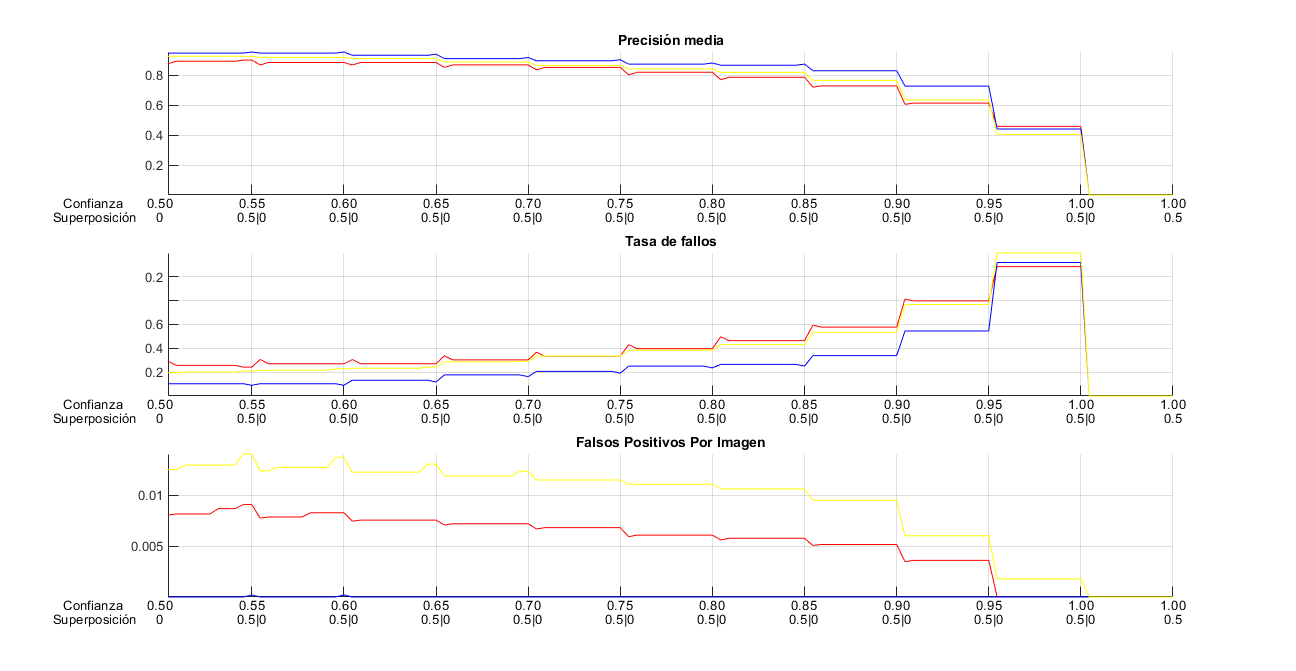
\includegraphics[width=1\textwidth]{Segmentacion con redes neuronales/YOLO/evaluacion LEGONet.png}
	\caption{Evaluación de YOLO basado en LEGONet en función de diversos parámetros}
	\label{fig:YOLO LEGONet evaluacion}
\end{figure}

Analizando estos resultados, se ha determinado que un buen punto de compromiso entre precisión, tasa de fallos y falsos positivos se obtiene con un límite de incertidumbre de 0.55 y un factor de superposición de 0.15. En los resultados mostrados a continuación se ha trabajado en este punto de operación. Tras analizar observamos que todas las gráficas presentan mejores resultados frente a Faster R-CNN basado en LEGONet y que todas las gráficas presenta distribuciones usuales. Esto es más notable en el caso de las piezas amarillas y rojas.

\begin{itemize}
\item Amarillo: El error cometido al detectar las piezas tanto en precisión como en fallos y falsos positivos en moderadamente elevado. Analizando las gráficas vemos que el número de falsos positivos no es elevado y sin embargo la tasa de fallos es elevada. Además, se observa en las gráficas que los cambios son abruptos y escasos, esto se debe a que el sistema apenas ha tenido falsos positivos lo cual también implica que la exhaustividad apenas varía.
\item Rojo: El rojo presenta una situación similar al amarillo. No presenta una tasa de falsos positivos elevada pero la tasa de fallos es más elevada. Como consecuencia, la precisión es más baja.
\item Azul: El azul presenta los mejores resultados de los tres, pero en las gráficas no se refleja esta situación. Esto se debe a que al analizar las imágenes no ha habido ningún falso positivo y por ello la precisión no varía con la exhaustividad y tampoco la tasa de fallos con los falsos positivos.
\end{itemize}

Analizando los resultados en conjunto se puede ver que la red ha tenido problemas para distinguir las piezas amarillas y rojas ya que en determinadas situaciones estas no han sido detectadas debido a cambios de iluminación. Aun así supone un gran avance frente a Faster R-CNN basado en LEGONet. Se puede observar una mejor comparación entre todos los métodos en el \autoref{chap:Resultados}.

\begin{figure}[ht]  %Estudio Amarillo
  \subfloat{
	\begin{minipage}[c][1\width]{0.49\textwidth}
	   \centering
	   \includegraphics[width=1\textwidth]{Segmentacion con redes neuronales/YOLO/precision yellow legonet.png}
	\end{minipage}}
  \hfill	
  \subfloat{
	\begin{minipage}[c][1\width]{0.49\textwidth}
	   \centering
	   \includegraphics[width=1\textwidth]{Segmentacion con redes neuronales/YOLO/miss yellow legonet.png}
	\end{minipage}}
\caption{Estudio de la segmentación por YOLO basado en LEGONet al detectar piezas amarillas}
\label{fig:yellow YOLO LEGONet}
\vspace{-5pt}
\end{figure}

\begin{figure}[ht]  %Estudio Rojo
  \subfloat{
	\begin{minipage}[c][1\width]{0.49\textwidth}
	   \centering
	   \includegraphics[width=1\textwidth]{Segmentacion con redes neuronales/YOLO/precision red legonet.png}
	\end{minipage}}
  \hfill	
  \subfloat{
	\begin{minipage}[c][1\width]{0.49\textwidth}
	   \centering
	   \includegraphics[width=1\textwidth]{Segmentacion con redes neuronales/YOLO/miss red legonet.png}
	\end{minipage}}
\caption{Estudio de la segmentación por YOLO basado en LEGONet al detectar piezas rojas}
\label{fig:red YOLO LEGONet}
\vspace{-5pt}
\end{figure}

\begin{figure}[ht]  %Estudio Azul
  \subfloat{
	\begin{minipage}[c][1\width]{0.49\textwidth}
	   \centering
	   \includegraphics[width=1\textwidth]{Segmentacion con redes neuronales/YOLO/precision blue legonet.png}
	\end{minipage}}
  \hfill	
  \subfloat{
	\begin{minipage}[c][1\width]{0.49\textwidth}
	   \centering
	   \includegraphics[width=1\textwidth]{Segmentacion con redes neuronales/YOLO/miss blue legonet.png}
	\end{minipage}}
\caption{Estudio de la segmentación por YOLO basado en LEGONet al detectar piezas azules}
\label{fig:blue YOLO LEGONet}
\vspace{-5pt}
\end{figure}

\newpage
\subsection{YOLO basado en LEGO16}
LEGO16 cuenta con un total de 41 capas, 13 son capas de convolución y 3 son completamente conectadas. En total cuenta con 138 millones de parámetros y 13 millones de neuronas. Frente a LEGONet, se trata de una red grande y pesada que requiere de más tiempo y potencia para ser entrenada,por suerte YOLO es bastante rápida para entrenar y esto no supone un gran problema. Pero antes es necesario modificar la para transformarla en una red tipo YOLO.

\subsubsection*{Estructura}
Como ya se ha visto en la anterior sección, YOLO se caracteriza por no funcionar como un clasificador. Esto implica que es necesario cambiar el final del clasificador añadiendo más capas de convolución y una capa de transformación y otra de salida. Estas capas se van a añadir a partir de la capa ReLu5\_3 que es la capa \textit{ReLu} de la última capa de convolución. Se puede observar la estructura final empleada para el entrenamiento en la \autoref{fig:YOLO LEGO16 estructura}.

\begin{figure}[ht]  %Estructura YOLO basado en LEGO16
	\centering
	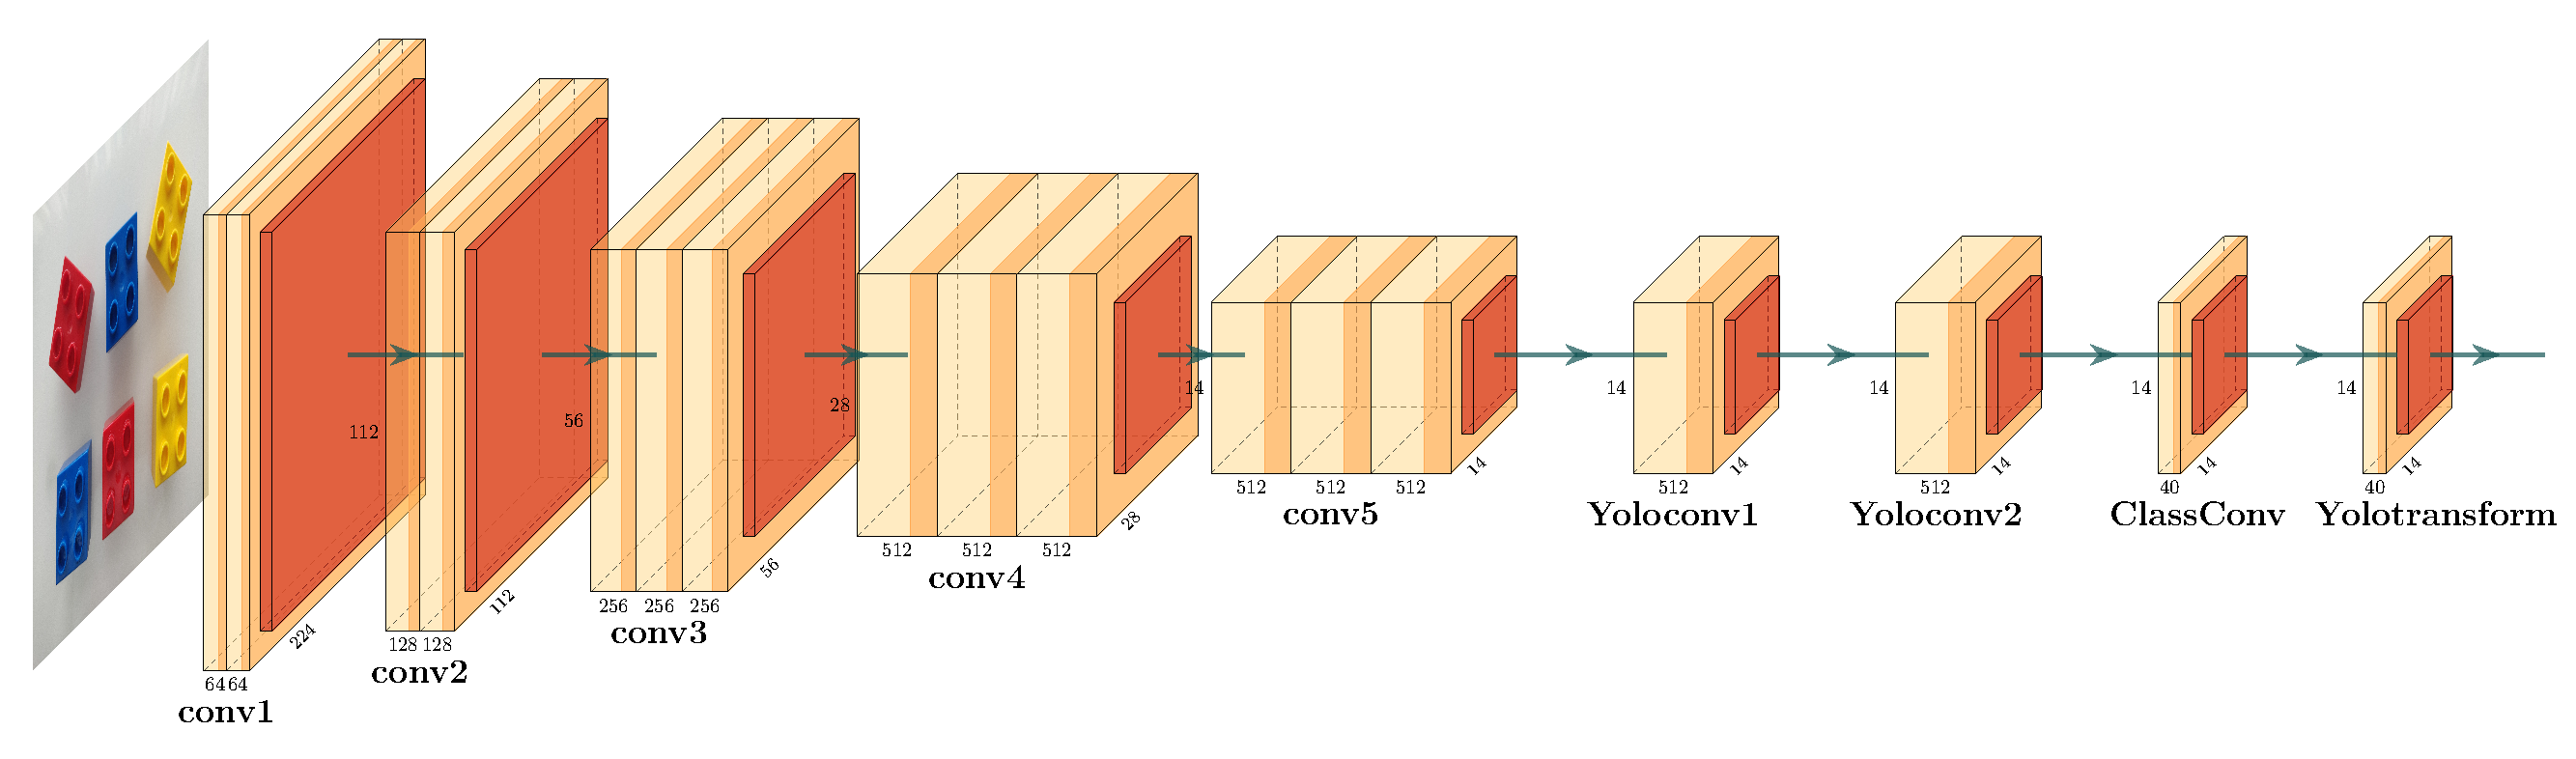
\includegraphics[width=0.8\textwidth]{Segmentacion con redes neuronales/YOLO/YOLO_LEGO16.pdf}
	\caption{Estructura de YOLO basado en LEGO16}
	\label{fig:YOLO LEGO16 estructura}
\end{figure}

\subsubsection*{Entrenamiento}
Para el entrenamiento de esta red se ha usado la base de datos diseñada en la \autoref{sec:Preparativos para el de entrenamiento detectores}. Esta base de datos consta de un total de 2.076 imágenes con un total de 5.886 piezas de LEGO. Se han realizado numerosas pruebas de entrenamiento y se ha descubierto que las mejores opciones de entrenamiento son las mostradas en la \autoref{tab:YOLO LEGO16 options}.

\begin{table}[ht]
  \centering
    \begin{tabular}{|l|c|}
    \hline
    \multicolumn{2}{|c|}{Opciones de entrenamineto} \\
    \hline
    Optimizador & \multicolumn{1}{l|}{Stochastic Gradient Descent with Momentum (SGDM)} \\
    \hline
    Momentum & 0.9 \\
    \hline
    Initial Learn Rate & 1.00E-03 \\
    \hline
    Learn Rate Schedule & piecewise \\
    \hline
    Learn Rate Drop Factor & 0.1 \\
    \hline
    Learn Rate Drop Period & 50 \\
    \hline
    L2Regularization & 0.004 \\
    \hline
    Max Epochs & 100 \\
    \hline
    Mini Batch Size & 25 \\
    \hline
    Shuffle data & every epoch \\
    \hline
    \end{tabular}%
  \caption{Opciones de entrenamiento de YOLO basado en LEGO16}
  \label{tab:YOLO LEGO16 options}%
\end{table}%


\subsubsection*{Resultados}
Con la ayuda del \textit{script} definido en la \autoref{subsec:evaluacion}, se han podido obtener cuatro parámetros que permiten evaluar la capacidad de esta red: tasa de fallos, falsos positivos por imagen (FPPI), precisión de los \textit{bounding boxes} y la exhaustividad. Al correr un detector de objetos existen múltiples parámetros a definir por el usuario que marcan el comportamiento de la red. Se ha evaluado la red con todas las posibles combinaciones de parámetros lógicas y se ha determinado el mejor rango de funcionamiento de la red. Estos parámetros son el nivel de superposición de las \textit{bounding boxes} y el límite de incertidumbre aceptable para determinar que lo detectado es un objeto. Al analizar todos los casos lógicos se han obtenido los resultados mostrados en la \autoref{fig:YOLO LEGO16 evaluacion}. En el eje x se puede ver los casos que se han analizado. El umbral de confianza se ha variado desde 0.5 hasta 1 en intervalos de 0.05 y para cada caso se ha evaluado modificando el nivel de superposición entre \textit{bounding boxes}. El nivel de superposición se ha variado entre 0 y 0.5 con intervalos de 0.05.

\begin{figure}[ht]  %Evaluación de YOLO basado en LEGO16
	\centering
	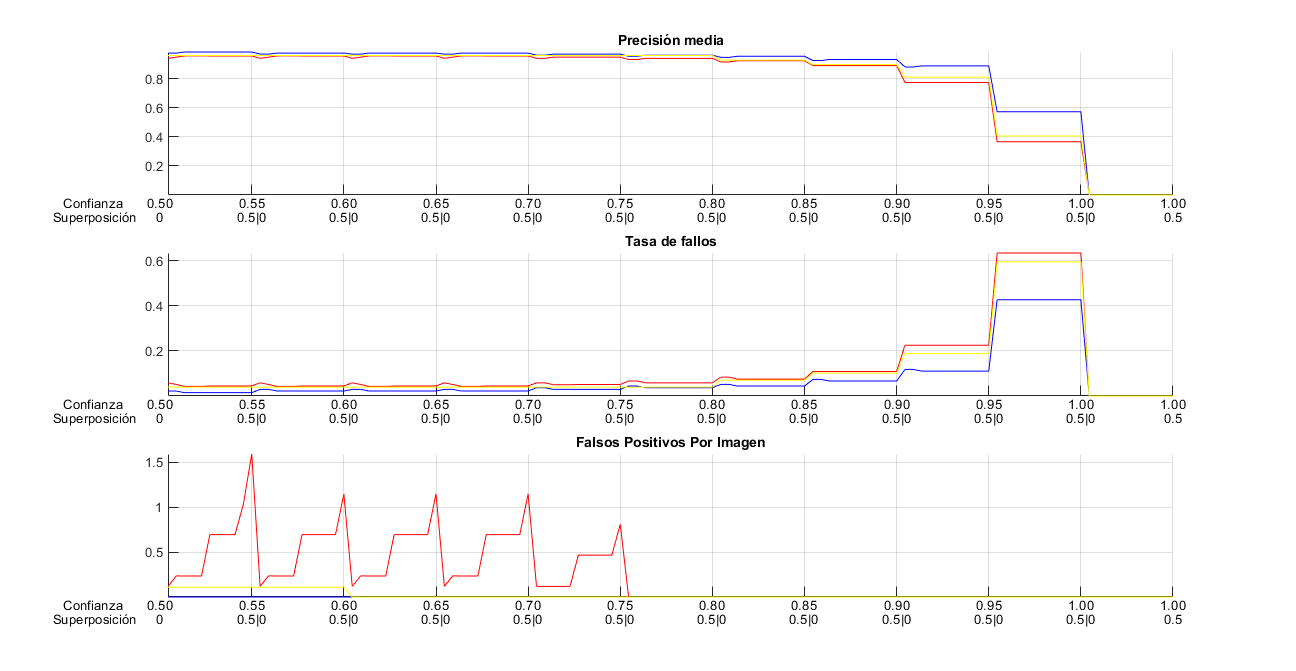
\includegraphics[width=1\textwidth]{Segmentacion con redes neuronales/YOLO/evaluacion LEGO16.png}
	\caption{Evaluación de YOLO basado en LEGO16 en función de diversos parámetros}
	\label{fig:YOLO LEGO16 evaluacion}
\end{figure}

Analizando estos resultados, se ha determinado que un buen punto de compromiso entre precisión, tasa de fallos y falsos positivos se obtiene con un límite de incertidumbre de 0.75 y un factor de superposición de 0.2.  Para los resultados mostrados a continuación se ha trabajado en este punto de operación.

Analizando estos resultados, se ha determinado que un buen punto de compromiso entre precisión, tasa de fallos y falsos positivos se obtiene con un límite de incertidumbre de 0.60 y un factor de superposición de 0.2. En los resultados mostrados a continuación se ha trabajado en este punto de operación. Tras analizar observamos que todas las gráficas presentan mejores resultados frente a YOLO basado en LEGONet. A pesar de que los resultados son muy positivos, las gráficas no lo reflejan correctamente debido a la falta de puntos para mostrar. Los falsos positivos han sido muy escasos y por ello hay tan pocos puntos y las gráficas son tan abruptas.

\begin{itemize}
\item Amarillo: El error cometido al detectar las piezas tanto en precisión como en fallos y falsos positivos en bastante bajo. Analizando las gráficas vemos que la tasa de fallos no es elevada y que no se ha dado ningún caso con falsos positivos. La precisión es muy elevada y aunque parece que se mantiene constante en 1, esto no es así ya que ha habido casos en los que no se han detectado las piezas rojas. Por ello la precisión media es inferior al 100\%.
\item Rojo: El rojo presenta una situación similar al amarillo. Presenta una tasa de fallos baja y una precisión elevada y a diferencia del amarillo, sí que presenta falsos positivos, aunque muy bajo.
\item Azul: El azul presenta los mejores resultados de los tres, pero en las gráficas no se refleja esta situación. Esto se debe a que al analizar las imágenes no ha habido ningún falso positivo y por ello la precisión no varía con la exhaustividad y tampoco la tasa de fallos.
\end{itemize}

Analizando los resultados en conjunto se puede ver la superioridad de VGG-16 frente a AlexNet y la capacidad de YOLO. Se puede observar una mejor comparación entre todos los métodos en el \autoref{chap:Resultados}.

\begin{figure}[ht]  %Estudio Amarillo
\vspace{-30pt}
  \subfloat{
	\begin{minipage}[c][1\width]{0.49\textwidth}
	   \centering
	   \includegraphics[width=1\textwidth]{Segmentacion con redes neuronales/YOLO/precision yellow lego16.png}
	\end{minipage}}
  \hfill	
  \subfloat{
	\begin{minipage}[c][1\width]{0.49\textwidth}
	   \centering
	   \includegraphics[width=1\textwidth]{Segmentacion con redes neuronales/YOLO/miss yellow lego16.png}
	\end{minipage}}
\caption{Estudio de la segmentación por YOLO basado en LEGO16 al detectar piezas amarillas}
\label{fig:yellow YOLO LEGO16}
\vspace{-5pt}
\end{figure}

\begin{figure}[ht]  %Estudio Rojo
\vspace{-30pt}
  \subfloat{
	\begin{minipage}[c][1\width]{0.49\textwidth}
	   \centering
	   \includegraphics[width=1\textwidth]{Segmentacion con redes neuronales/YOLO/precision red lego16.png}
	\end{minipage}}
  \hfill	
  \subfloat{
	\begin{minipage}[c][1\width]{0.49\textwidth}
	   \centering
	   \includegraphics[width=1\textwidth]{Segmentacion con redes neuronales/YOLO/miss red lego16.png}
	\end{minipage}}
\caption{Estudio de la segmentación por YOLO basado en LEGO16 al detectar piezas rojas}
\label{fig:red YOLO LEGO16}
\vspace{-5pt}
\end{figure}

\begin{figure}[ht]  %Estudio Azul
\vspace{-30pt}
  \subfloat{
	\begin{minipage}[c][1\width]{0.49\textwidth}
	   \centering
	   \includegraphics[width=1\textwidth]{Segmentacion con redes neuronales/YOLO/precision blue lego16.png}
	\end{minipage}}
  \hfill	
  \subfloat{
	\begin{minipage}[c][1\width]{0.49\textwidth}
	   \centering
	   \includegraphics[width=1\textwidth]{Segmentacion con redes neuronales/YOLO/miss blue lego16.png}
	\end{minipage}}
\caption{Estudio de la segmentación por YOLO basado en LEGO16 al detectar piezas azules}
\label{fig:blue YOLO LEGO16}
\vspace{-5pt}
\end{figure}